\documentclass{fhnwreport/fhnwreport}

\usepackage{lipsum}
\usepackage[english]{babel}
\usepackage{tikz}
\usetikzlibrary{arrows}
\usetikzlibrary{patterns}
\usetikzlibrary{plotmarks}
%\pgfplotsset{try min ticks=3}
\usepackage{pgfplots}
\pgfplotsset{compat=newest}
\pgfplotsset{max space between ticks=80pt}
\pgfplotsset{max space between ticks=80pt}
\pgfplotsset{
    tick label style={font=\small},
    label style={font=\small},
    legend style={font=\footnotesize}
}
\usepackage[T1]{fontenc}
%\usepackage{textcomp}
%\usepackage[utf8x]{inputenc}
\usepackage[utf8]{inputenc}
\usepackage{amsmath}
\usepackage{amsfonts}
%\usepackage{MnSymbol}
\usepackage{wasysym}
\usepackage{lmodern}   %Type1-Schriftart f\"ur nicht-englische Texte
\usepackage{datetime}
\usepackage{cite}
\usepackage{lipsum}
\usepackage{booktabs}
\usepackage{pdflscape}
\usepackage{longtable}
\usepackage[figuresright]{rotating} % for single-sided printing
\usepackage{xcolor}
\usepackage{colortbl}
\usepackage{hyperref}
\usepackage[titletoc,title]{appendix}
\usepackage{graphicx}
\usepackage{pdfpages}
\usepackage{enumitem}
\usepackage{caption}
\usepackage{gensymb}
\usepackage{pbox}
%\usepackage{draftwatermark}
%\usepackage[nostamp]{draftwatermark}
\usepackage[textsize=footnotesize, textwidth = 17mm, german, colorinlistoftodos]{todonotes}
\usepackage[separate-uncertainty = true]{siunitx}
\usepackage{mathtools}
\usepackage{matlab-prettifier}
\usepackage{spreadtab}
\usepackage{transparent}
\usepackage{relsize}
\usepackage{svg}
\usepackage{multirow}
\usepackage{csquotes}
\usepackage{wrapfig}
%\usepackage[style=mla,backend=bibtex]{biblatex}
%\addbibresource{bibliography/bibliography.bib}

\definecolor{dkgreen}{rgb}{0,0.6,0}
\definecolor{gray}{rgb}{0.5,0.5,0.5}
\definecolor{mauve}{rgb}{0.58,0,0.82}

\lstdefinestyle{java}{
    language            = Java,
    aboveskip           = 3mm,
    belowskip           = 3mm,
    showstringspaces    = false,
    columns             = flexible,
    basicstyle          = {\scriptsize\ttfamily},
    numbers             = left,
    numberstyle         = \tiny\color{gray},
    keywordstyle        = \color{blue},
    commentstyle        = \color{dkgreen},
    stringstyle         = \color{mauve},
    breaklines          = true,
    breakatwhitespace   = true,
    tabsize             = 3
}
\lstdefinestyle{Matlab-editor-2}{%
  style               = MatlabBaseStyle@mlpr,
  mllastelementstyle  = \color{black}                    ,
  mlkeywordstyle      = \color[RGB]{000,000,255}         ,
  mlcommentstyle      = \color[RGB]{034,139,034}         ,
  mlstringstyle       = \color[RGB]{160,032,240}         ,
  mlsyscomstyle       = \color[RGB]{178,140,000}         ,
  mlsectiontitlestyle = \commentStyle@mlpr      \bfseries,
  mlsharedvarstyle    = \color[RGB]{000,163,163}         ,
  mlplaceholderstyle  = \mleditorphstyle,
  basicstyle          = \ttfamily\scriptsize,
  numbers             = left,
}


%\SetWatermarkText{\texttt{Entwurf}}
%\SetWatermarkText{Entwurf}
%\SetWatermarkLightness{0.9}

\setcounter{secnumdepth}{5} % up to and including paragraph. Not working atm.
\setcounter{tocdepth}{2}

\DeclarePairedDelimiter\abs{\lvert}{\rvert}%

%\renewcommand{\thesubsubsection}{\arabic{subsubsection}}

%\renewcommand{\thefootnote}{\roman{footnote}}
\renewcommand{\thefootnote}{\Roman{footnote}}

\hypersetup{%
  bookmarksnumbered = true,
  colorlinks = true,
  linkcolor  = black,
  citecolor  = black,
  %urlcolor   = blue,
  urlcolor   = black,
  %hidelinks  = false
}

\author{%
    Frey, Raphael\\
    \texttt{raphael.frey@students.fhnw.ch}
    \and
    Freivogel, Reto\\
    \texttt{reto.freivogel@students.fhnw.ch}
    \and
    Murray, Alex\\
    \texttt{alexander.murray@students.fhnw.ch}
}

\title{%
    \textbf{\Huge{\texttt{BAT6}}} \\
}

%\newcommand{\colfigure}[3]{%
    \begin{minipage}[c][][b]{0.485\textwidth}
        #1
    \end{minipage}
    \hspace{0.03\textwidth}
    \begin{minipage}[c][][b]{0.485\textwidth}
        {\raggedleft%
            \includegraphics[width=0.9\textwidth]{#2}%
        }
        \captionof{figure}{#3}
    \end{minipage}\\%
}

%\newlist{longenum}{enumerate}{5}
\setlist[longenum,1]{label=\roman*)}
\setlist[longenum,2]{label=\alph*)}
\setlist[longenum,3]{label=\arabic*)}
\setlist[longenum,4]{label=(\roman*)}
\setlist[longenum,5]{label=(\alph*)}

\def\code#1{\texttt{#1}}

\DeclareSIUnit[number-unit-product = {}]
    \partspermillion{ppm}
\DeclareSIUnit[number-unit-product = {}]
    \permille{\perthousand}



\begin{document}

\begin{titlepage}

    \maketitle
    \vspace{40mm}
    \begin{center}
        \Large{Solar Panel Emulator}%
    \end{center}

    \vspace{50mm}
    %\vspace{90mm}

    %\hspace{-20mm}
    \begin{tabular}{r|l}

        \textsc{\textbf{Degree Program}}
        & EIT\\
        [4mm]

        \textsc{\textbf{Module}}
        & Projekt 3 \\
        [4mm]

        \textsc{\textbf{Team}}
        & 2 \\
        [4mm]

        \textsc{\textbf{Sponsor}}
        & Hanspeter Gysin \\
        [4mm]

        \textsc{\textbf{Coaches}}
        & Hanspeter Gysin, Peter Ganzmann, Matthias Meier,\\
        & Anita Gertiser, Bonnie Domenghino\\
        [4mm]

        %\textsc{\textbf{A}}
        %& Reto Freivogel, Alexander Murray, Raphael Frey\\
        %[4mm]

        \textsc{\textbf{Version}}
        & \code{1} \\
    \end{tabular}
    %\end{center}

\end{titlepage}


% **************************************************************************** %
\clearpage
\pagestyle{empty}
{
    \section*{Abstract}
    \label{sec:abstract}
% **************************************************************************** %
    % relevance/motivation
% problem statement
% approach: how is the problem solved
% results
% conclusions
% keywords

% introduction
% research problem
% body
% results
% conclusion

 % introduction
Emulating  solar  modules  in  a  laboratory  environment  currently  requires
expensive  and complex  equipment, hindering  development of  new solar  power
products. To  facilitate research  into  this area,  a  low-cost solution  for
emulating solar modules is required.

% approach
This report details our efforts in designing and constructing  a device for this
purpose.   We   developed   a   model  for  describing  solar  module   behavior
mathematically,  allowing both single-celled panels  as  well  as  more  complex
multi-celled panel configurations  to  be  described.  A  microcontroller  and a
voltage  converter  constitute  the  hardware  design.  The  microcontroller  is
responsible  for interacting with  the  outside  world,  while  the  converter's
purpose is to use the mathematical model  to  generate  the desired voltages and
currents on the device's output.

% results
At this point, the interface  and  most  of  the  circuitry  works  as intended.
Unfortunately,  due  to  a  design  error,  our  circuit  overloads  the voltage
converter, causing irreparable damage. Based on measurements and simulations, we
consider the likely cause to be overlong connections between  the  converter and
other components. The next step in finalising the device would  be  to  design a
new circuit board for fixing this issue.


}


% **************************************************************************** %
\clearpage
\pagestyle{empty}
{
    \renewcommand{\thispagestyle}[1]{}
    \tableofcontents
    %\vspace{35mm}
    %\subsection*{Versionsgeschichte}
    %\begin{itemize}
    %    \item[]
    %        %\emph{20.10.2015:} \texttt{Version 1}
    %        \emph{10th Oct 2015:} \texttt{Version 0.1:} Einleitung \& Disposition
    %    \item[]
    %        \emph{2nd Jan 2015:} \texttt{Version 0.2:} Translation to English
    %\end{itemize}
}

\clearpage
\setcounter{page}{1}
\pagestyle{headings}
% **************************************************************************** %

% **************************************************************************** %
\clearpage
\section{Introduction}
\label{sec:introduction}
% **************************************************************************** %
% Structured according to Gertiser's feedback:
% 1) Worum geht es?
% 2) Ziel und Anforderungen
% 3) Umsetzung -> Grobkonzept
% 4) Resultate
% 5) Aufbau der Arbeit

% TODO: source for expensive shit

Verifying the correct operation of equipment  used for testing solar arrays is
currently difficult in  a controlled laboratory environment,  as no affordable
solutions for this exist on the open market. To address this issue, the aim of
this project was the development of a device capable of emulating the behavior
of a  photovoltaic module. With this  device, test equipment  for photovoltaic
modules can be verified to function  as specified in a laboratory conveniently
and affordably.

The primary characteristics  of our device should be compactness  (usable in a
standard  laboratory environment),  the  capability to  emulate varying  solar
irradiation levels,  being able  to be  used in  series with  other emulators,
effiency with  regards to  power consumption  and losses,  and to  emulate the
characteristic  curve of  an actual  PV module. A  more detailed  list of  the
technical  requirements  can be  found  in  the specifications  (see  appendix
\ref{appendix:specs} on page \pageref{appendix:specs}f)

A microcontroller and a constant-current, constant-voltage step-down converter
constitute the core of our device.  The microcontroller performs IO operations
and implements  the regulation loop  used to control the  step-down converter,
whereas  the  step-down converter  generates  the  output voltage  and  output
current  corresponding  to  the  desired  operating  point  from  a  DC  power
supply. The  entire design  is  based  around a  custom  PCB,  enabling us  to
optimise impedances of  connections between critical components. Additionally,
we can get very close in behavior to a potentially mass-produced product since
trace lenghts, routing  and component placement are crucial  (see also section
\ref{sec:verification}, beginning on page \pageref{sec:verification}).

The device has a simple yet powerful user interface which can be controlled by
a push-twist button and a modern OLED display. The device can also be remotely
monitored and controlled from a PC via USB interface and custom software built
on the  Qt application framework  and is  compatible with all  major operating
systems~\cite{ref:qt}.  Our  device can emulate fairly  complex configurations
of cells thanks to an efficient  use of computation resources and its powerful
microprocessor.

Section  \ref{sec:concept}   (p.  \pageref{sec:concept}ff)  of   this  reports
deal  with   the  basic  concept  behind   our  solution. Component  selection
and   PCB  design   are  documented   in  sections   \ref{sec:components}  (p.
\pageref{sec:components}ff)   and   \ref{sec:pcb}  (p.   \pageref{sec:pcb}ff),
respectively,   while    section   \ref{sec:software}   is    concerned   with
software  (p. \pageref{sec:software}ff).   Section \ref{sec:verification}  (p.
\pageref{sec:verification}ff)  deals with  testing  the device  and our  error
analysis. Lastly, the conclusion can  be found in section \ref{sec:conclusion}
on page \pageref{sec:conclusion}.


% **************************************************************************** %
%\clearpage
%\section{Task Description}
%\label{sec:task}
%% **************************************************************************** %
%\begin{itemize}
    \item
        Was ist der grunds\"atzliche Auftrag?
    \item
        Was ist das Ziel?
    \item
        Motivation hinter dem Projekt/Auftrag?
    \item
        Grunds\"atzliche  Informationen  zu  Photovoltaik-Modulen und  den  zu
        untersuchenden  Fragen  (Verhalten  unter  nicht-idealen  Umst\"anden)
        liefern.
    \item
        Was sind die grunds\"atzlichen Anforderungen an unser Ger\"at?
\end{itemize}



% **************************************************************************** %
\clearpage
\section{Basic Concept}
\label{sec:concept}
% **************************************************************************** %
%\begin{itemize}
%    \item
%        Weshalb wurde das benutzte mathematische Modell gew\"ahlt?
%    \item
%        Weshalb wird ein Schaltregler benutzt?
%    \item
%        Weshalb wurde ein eigenes PCB entwickelt statt ein Steckbrett verwendet?
%    \item
%        Wie soll unser Ger\"at bedient werden k\"onnen?
%\end{itemize}

This section primarily deals with the underlying mathematics used to model the
various  configurations  of  solar  cells  the device  needs  to  be  able  to
emulate. Additionally, it presents a brief overview of the hardware.

% **************************************************************************** %
\subsection{The Model}
% **************************************************************************** %

The aim in developing  our model was to find the  sweet spot between usability
and  accuracy. It  should  have  a  small,  comprehensive  set  of  parameters
which  can be  easily understood  by the  user, while  still representing  the
actual physics  accurately enough to  yield good results.


% **************************************************************************** %
\subsubsection{Single Solar Cell}
% **************************************************************************** %

\begin{minipage}{0.6\textwidth}
    The single diode model of the ideal PV cell\cite{ref:villa:pvmodel} serves
    as  a basis  for our  model.   The I-V  characteristic of  this model  can
    be  expressed  with equation  \ref{eq:I-V_old},  whereby  $I_{pv}$ is  the
    generated current,  $I_o$ is the diode  current and $ V_T$  is the thermal
    voltage.
\end{minipage}
\begin{minipage}{0.4\textwidth}
    \begin{equation} \label{eq:I-V_old}
        I = I_{pv} - I_o \left[ \exp \left( \frac{V}{V_T} \right) - 1 \right]
    \end{equation}
\end{minipage}

\begin{minipage}{0.7\textwidth}
    Although these  three parameters depend  on the junction  temperature, the
    inclusion  of the  junction  temperature  into our  model  as a  parameter
    would  only  contribute a  minor  correction  factor, negligible  for  our
    purposes.  For this reason we can simplify our model if we assume that the
    temperature is equal to the nominal temperature $T_n = 298.15K$.

    The  thermal  voltage  is  defined  in  equation  \ref{eq:thermalvoltage},
    whereby $T$ is the junction temperature, $k$ is the Boltzman constant, $q$
    is  the elementary  charge and  $a$ is  the diode  ideality factor,  which
    typically  lies around  1.2  for silicon  substrates. This  gives us  $V_T
    \approx 30.8mV$ for one cell.

    The  current generated  by the  cell is  calcualted according  to equation
    \ref{eq:cellcurrent}, whereby $I_n$  is the nominal current  and $G$ and
    $G_n$ is the actual and nominal solar irradiation, respectively.

    A  common optimisation,  according to\cite{ref:villa:pvmodel},  is to  set
    $I_n \approx  I_{sc}$ and  again assume that  the temperature  is constant
    ($T  =  T_n$),   giving  us  $\Delta_T  =  0$   and  simplifying  equation
    \ref{eq:cellcurrent} to equation \ref{eq:I_pv}.

    Finally, the diode  leakage current at the nominal  temperature (for other
    temperatures  please  see  \cite{ref:villa:pvmodel})  is  calculated  with
    equation \ref{eq:I_o}.

    If  we  insert  equations  \eqref{eq:I_o} and  \eqref{eq:I_pv}  back  into
    \eqref{eq:I-V_old} we get equation \ref{eq:IAlmostDone}.

    If   we  now   assume  $V_{oc}   >   5  \cdot   V_T$  we   can  say   that
    $e^{\frac{V_{oc}}{V_T}}-1  \approx e^{\frac{V_{oc}}{V_T}}$  and our  final
    formula becomes equation \eqref{eq:I-V}.
\end{minipage}
\begin{minipage}{0.3\textwidth}
    \begin{equation} \label{eq:thermalvoltage}
        V_T = a k T / q
    \end{equation}
    \begin{equation} \label{eq:cellcurrent}
        I_{pv} = \left( I_n + K_I \Delta_T \right) \frac{G}{G_n}
    \end{equation}
    \begin{equation} \label{eq:I_pv}
        I_{pv} = I_{sc} \frac{G}{G_n}
    \end{equation}
    \begin{equation} \label{eq:I_o}
        I_o = \frac{I_{sc}}{e^{V_{oc} / V_T} - 1}
    \end{equation}
    \begin{equation} \label{eq:IAlmostDone}
        I = I_{sc} \left( \frac{G}{G_n} - \frac{e^{\frac{V}{V_T}}-1}{e^{\frac{V_{oc}}{V_T}}-1} \right)
    \end{equation}
    \begin{equation} \label{eq:I-V}
        I = I_{sc} \left( \frac{G}{G_n} - e^{\frac{V - V_{oc}}{V_T}} \right)
    \end{equation}
\end{minipage}



% **************************************************************************** %
\subsubsection{Multiple Cells in Series}
% **************************************************************************** %

If the solar irradiation is the same  for  every  cell in series, then the whole
array  can be simulated using equation \eqref{eq:I-V}, where $V_{oc}$  and  $V_T$
are linearly scaled with the number of cells.

If the irradiation is not the same for all  cells,  such  as  when  one  cell  is
shaded, a more complex model must be used.

\begin{minipage}{0.5\textwidth}
    \center
    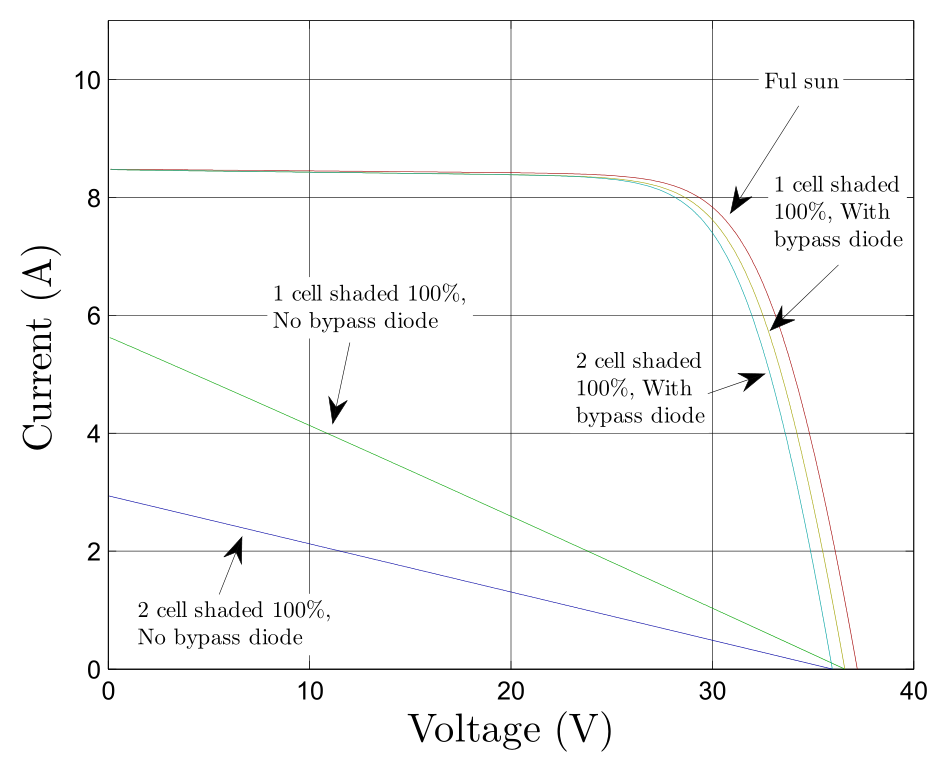
\includegraphics[width=\textwidth]{images/model/shaded.png}
    \captionof{figure}{I-V curves for different configurations and shaded cells\cite{ref:tian:model}}
    \label{fig:model:shaded}
\end{minipage}
\begin{minipage}{0.5\textwidth}
	\center
    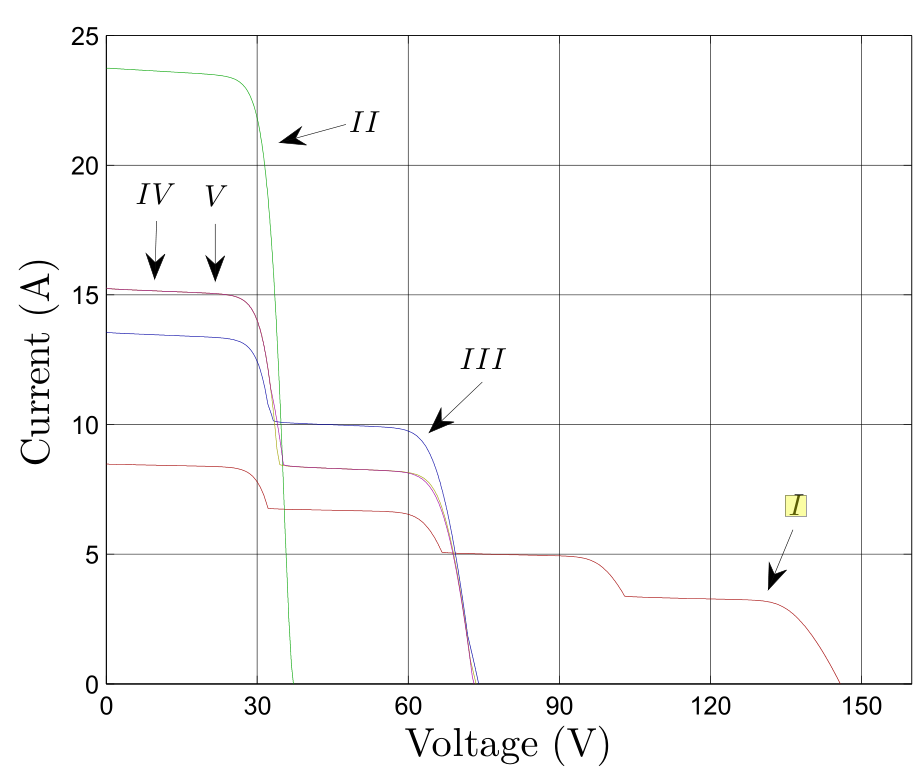
\includegraphics[width=\textwidth]{images/model/steps.png}
    \captionof{figure}{The typical characteristic of modules connected in series or in parallel}
    \label{fig:model:steps}
\end{minipage}


Figure \ref{fig:model:shaded} shows various  characteristic curves of a shaded
PV  module and  the effect  of bypass  diodes on  them.  In  our model  we can
emulate the I-V  curve of an array with  a shaded cell and no  bypass diode by
setting $V_T = V_{oc}$.

%Figure \ref{fig:model:shaded}  shows  what  varied  characteristics  of a shaded
%PV-module  look  like  and  how  bypass  diodes affect them. In our model we can
%imitate  the  I-V  curve of an array with a shaded cell and no bypass  diode  by
%setting $V_T = V_{oc}$.

The  characteristic  curves shown  in  Figure  \ref{fig:model:steps} show  how
``steps'' emerge when  two or more modules with bypass  diodes, which are each
exposed  to different  irradiation  intensities, are  connected in  series. To
emulate  this behaviour,  we take  a number  of curves  with decreasing  short
circuit current and increasing open  circuit voltage and determine which curve
is applicable by checking what curve returns the maximum current for the given
voltage.


% **************************************************************************** %
\subsection{Implementation of Regulation}
\label{subsec:regimplementation}
% **************************************************************************** %

To increase  accuracy in emulating  the I-V characteristic curve,  both output
voltage and output current of the  device's operating point are monitored.  If
the  operating  point  is  above  the  $-\frac{\SI{1}{\volt}}{\SI{1}{\ampere}}
=  \SI{-1}{\ohm}$ slope  (``A''  in figure  \ref{fig:controlcircuit:vicurve}),
more  accurate  regulation can  be  achieved  by  operating the  regulator  in
constant  current  mode.   In  contrast,  if  the  operating  point  is  below
the  \SI{-1}{\ohm} slope  (``B'' in  figure \ref{fig:controlcircuit:vicurve}),
operating the  regulator in constant voltage  mode will yield a  more accurate
result.

A       more        detailed       explanation       can        be       found
in      section       \ref{subsec:iv-curve-operating-points}      on      page
\pageref{subsec:iv-curve-operating-points}.

\begin{minipage}{0.5\textwidth}
    \center
    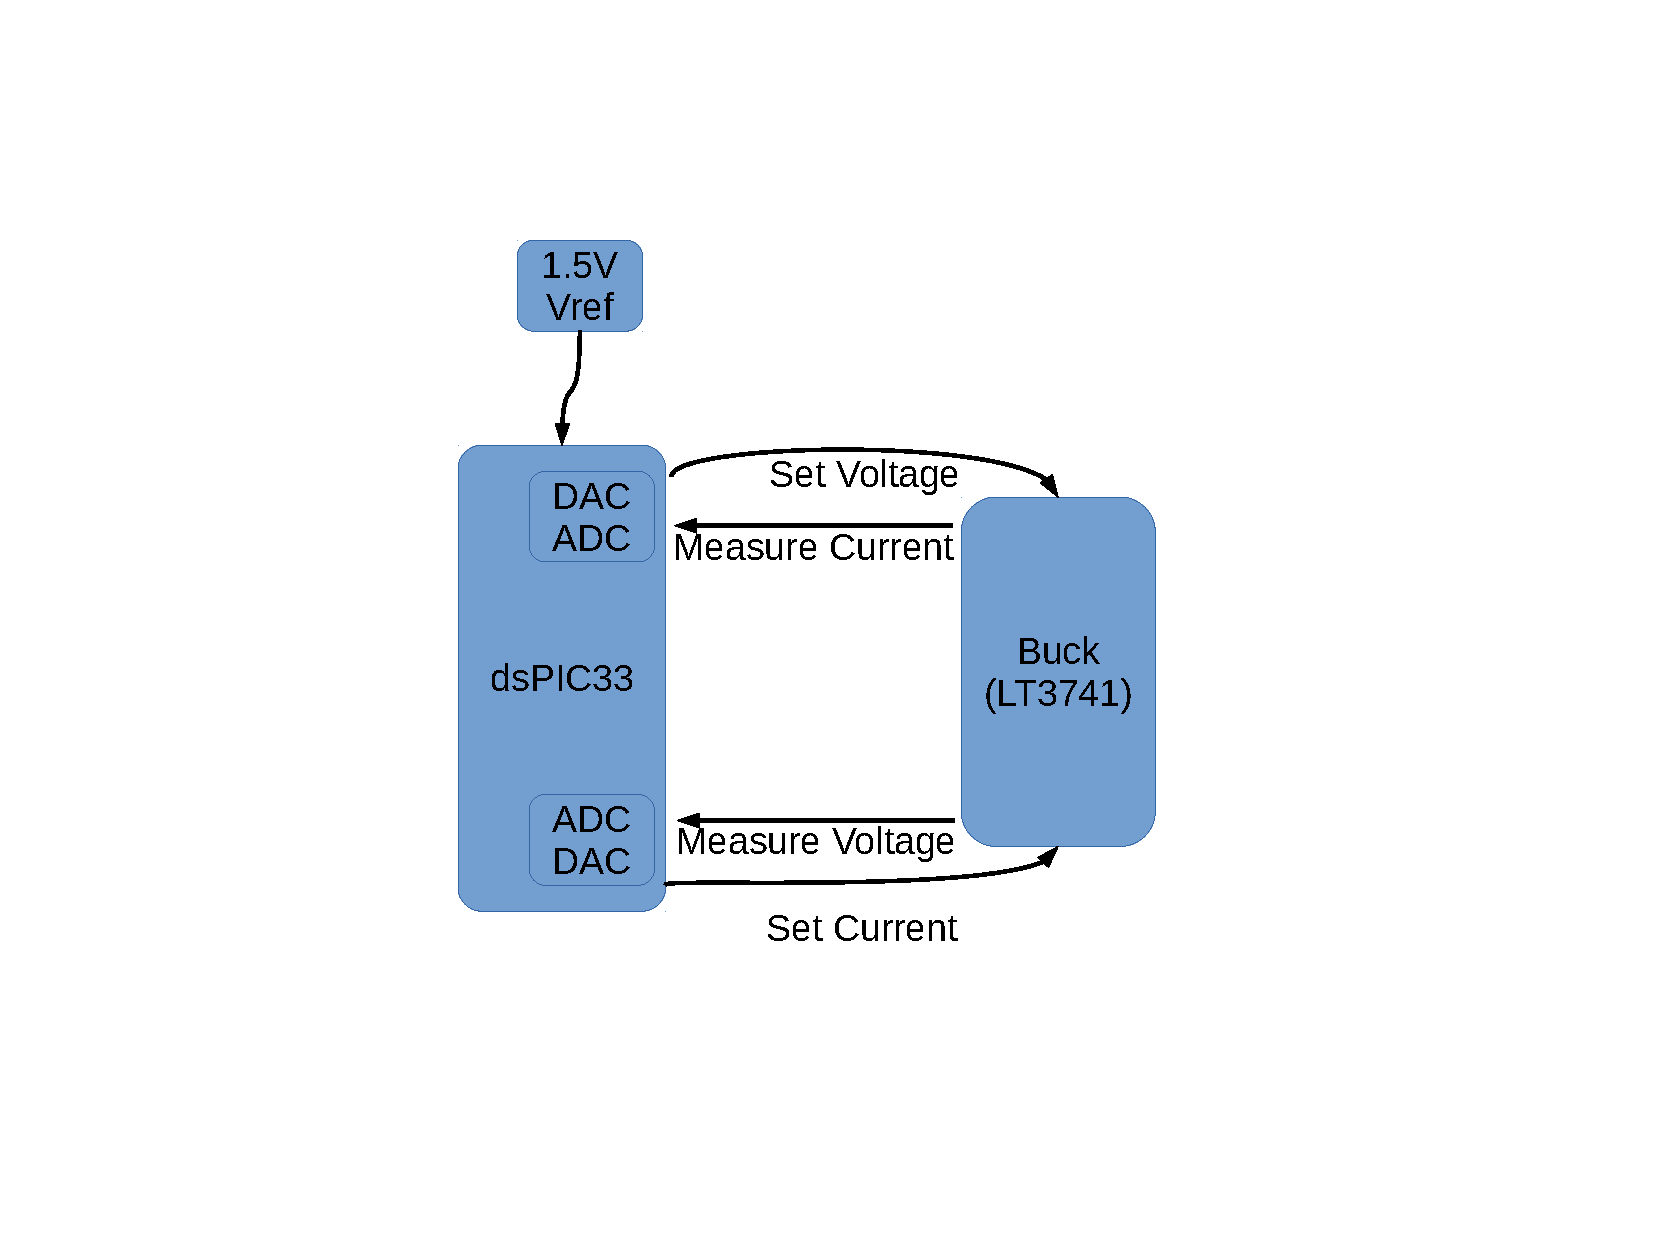
\includegraphics[width=\textwidth,trim=140 140 120 100,clip]{images/block-diag-control.pdf}
    \captionof{figure}{Block diagram of control circuit}
    \label{fig:controlcircuit:schcematic}
\end{minipage}
\begin{minipage}{0.5\textwidth}
    \center
    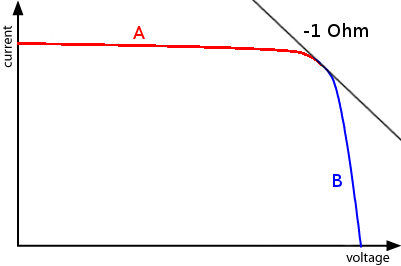
\includegraphics[width=\textwidth]{images/vi-curve.png}
    \captionof{figure}{I-V-Curve with \SI{-1}{\ohm} slope indicated}
    \label{fig:controlcircuit:vicurve}
\end{minipage}


% **************************************************************************** %
\subsection{Hardware}
% **************************************************************************** %

Our device is based  on a microcontroller, which is used  to handle user input
and output and  controls the step-down converter.  Power  delivery is realised
with a  prebuilt DC  power supply  unit. In addition  to interacting  with the
device directly, users can also connect a PC to our device by USB and then use
our front-end  software \emph{Smooth}  to interface  with the  device (section
\ref{subsec:frontend}, p. \pageref{subsec:frontend}ff).

With  an  eye  towards  potential  serial production,  we  developed  our  own
PCB. This  allows tight  control over  impedances in  the connections  between
critical  components  and   brings  the  behavior  of   the  prototype  device
much  closer   to  a  mass   produced  version  than  a   breadboard  solution
could. This  is because  trace  routing lengths  and  component placement  are
crucial  factors,  as  is  discussed  in  section  \ref{sec:verification}  (p.
\pageref{sec:verification}ff), \emph{Verification}.



% **************************************************************************** %
%\clearpage
\section{Component Selection}
\label{sec:components}
% **************************************************************************** %
In  this  section, the  selection  of  the  critical components  is  discussed
in  detail. Mainly,  this concerns  the  microcontroller,  the power  delivery
(both  external and  internal)  and  the circuitry  used  in conjunction  with
the  step-down converter. A  more comprehensive  list of  components including
costs can  be found  in appendix  \ref{appendix:components} beginning  on page
\pageref{appendix:components}. The complete schematics are located in appendix
\ref{appendix:schematics} on pages \pageref{appendix:schematics}ff.

%\begin{itemize}
%    \item
%        Was sind die Anforderungen an die Stromversorgung?
%    \item
%        Weshalb wird der dsPIC33EP-Chip verwendet?
%    \item
%        Weshalb wird der LT3741 verwendet?
%    \item
%        Wie erfolgt die Ansteuerung des LT3741?
%    \item
%        Weshalb wurde das verwendete LCD gew\"ahlt?
%    \item
%        Wie wird die serielle Schnittstelle realisiert?
%\end{itemize}

% **************************************************************************** %
\subsection{Microcontroller}
% **************************************************************************** %

Microchip  was chosen  as manufacturer  because one  of our  team members  was
already familiar  with their  products.  Additionally, Microchip  provides good
developer  tools  for free. For  selecting  a  specific model,  the  following
criteria eventually lead us to the \emph{dsPIC33EP16GS506}:

\begin{itemize}
    \item
        \SI{120}{\mega\hertz}  clock (60  MIPS): High enough  to allow  a fast
        control loop.
    \item
        2 ADCs  and 2  DACs with external  voltage reference: Required  by the
        control scheme  we use (see section  \ref{subsec:regimplementation} on
        \pageref{subsec:regimplementation}).
    \item
        PGA    (Programmable    Gain    Amplifier)   (64    $\times$    analog
        pre-amplifier): Allows     measuring     the    small     differential
        voltages     over    shunt     resistors    to     measure    currents
        (see     section      \ref{subsubsec:lt3741:feedback}     on     pages
        \pageref{subsubsec:lt3741:feedback}ff).
    \item
        Low cost of 4 CHF
\end{itemize}


% **************************************************************************** %
\subsection{36V Power Supply and Mains Input}
% **************************************************************************** %

The   maximum   required   output   power    of   our   device   was   roughly
calulated   as  $\SI{24}{\volt}   \cdot   \SI{3}{\ampere}  =   \SI{72}{\watt}$
(maximum  output   voltage  times  maximum   output  current,  based   on  the
VI-curve  in   the  specifications,   see  appendix   \ref{appendix:specs}  on
page  \pageref{appendix:specs}).   Assuming   an  efficiency  of  $\eta\approx
\SI{90}{\percent}$ an \SI{80}{W} power supply is therefore required.

We chose a power supply  capable of supplying \SI{28}{\volt} at \SI{75}{\watt}
and mounted  it inside the  case.  It  can be plugged  into a power  outlet by
means of an IEC  60320 C13 socket The socket has a built-in  fuse as well as a
built-in mains  filter, which  reduces high frequency  coupling back  into the
mains from the device.  A rocker switch is connected in series with the socket
and the power supply, allowing for the end user to cut power at any time.

%\ref{fig:circuit:mains-input}.
%
%\begin{figure}[th!]
%    \centering
%    \begin{minipage}{.3\textwidth}
%        \centering
%        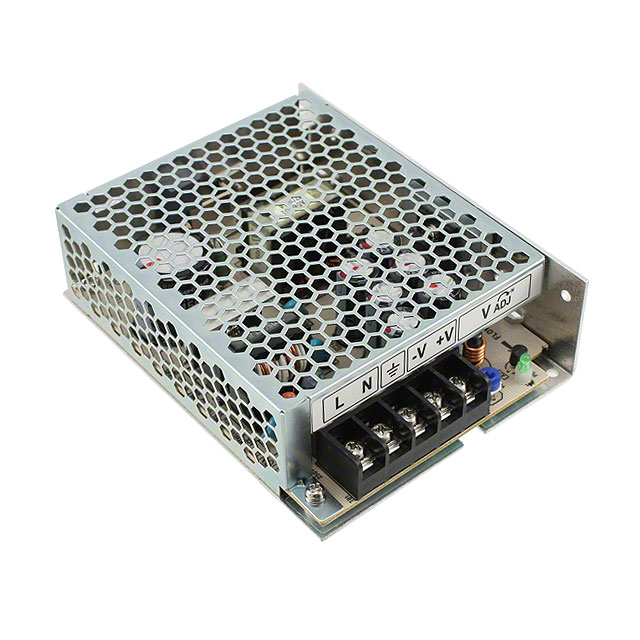
\includegraphics[width=\textwidth]{images/circuit/external-power-supply.JPG}
%        \caption{External PSU}
%        \label{fig:circuit:mains-input}
%    \end{minipage}
%    \begin{minipage}{.3\textwidth}
%        \centering
%        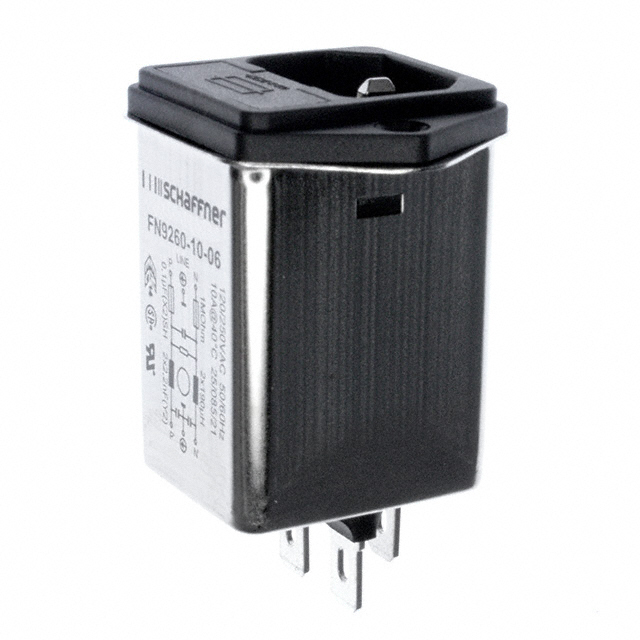
\includegraphics[width=.9\textwidth]{images/circuit/power-entry-module.JPG}
%        \caption{Power Entry Module}
%        \label{fig:circuit:iec60320c13}
%    \end{minipage}
%    \begin{minipage}{.3\textwidth}
%        \centering
%        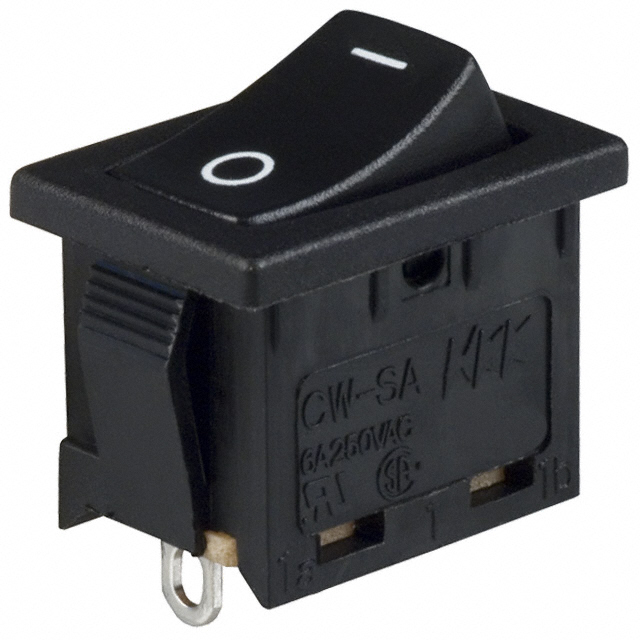
\includegraphics[width=.6\textwidth]{images/circuit/rocker-switch.JPG}
%        \caption{Rocker Switch}
%        \label{fig:circuit:rocker-switch}
%    \end{minipage}
%\end{figure}

%It can be plugged  into a power outlet by means of an  IEC 60320 C13 socket
% as seen in figure \ref{fig:circuit:iec60320c13}.
%The socket has a built-in fuse as  well as a built-in mains filter, which will
%reduce high frequency coupling back into the mains from the device.

%A rocker switch
%(figure \ref{fig:circuit:rocker-switch})
%is connected in series with the socket  and the power supply, allowing for the
%end user to cut power at any time.


% **************************************************************************** %
\subsection{Voltage Rails}
% **************************************************************************** %

\label{sec:voltage_rails}

In order to power the components  used in this design, three different voltage
rails are used: \SI{28}{\volt}, \SI{5}{\volt}  and \SI{3.3}{\volt}.  Each rail
has specific  requirements concerning electrical noise,  power and efficiency.
Selecting  appropriate  voltage  regulators requires  determining  approximate
values for the maximum current in each rail.

The power requirements on the \SI{3.3}{\volt} rail are primarily determined by
the dsPIC33  microcontroller and the  LEDs. For maximum processing  power, the
dsPIC33 will  be clocked  at its  maximum frequency  of \SI{120}{\mega\hertz},
consuming  \SI{0.5}{\milli\ampere\per\mega\hertz}  \cite{ref:datasheet:dspic}.
Each of the four LEDs consumes \SI{15}{\milli\ampere}.  This yields a combined
current consumption on the \SI{3.3}{\volt} rail of
\begin{equation}
    I_{\SI{3.3}{\volt}} = I_{dsPIC} + 4 \cdot I_{LED} = \SI{0.5}{\milli\ampere\per\mega\hertz} \cdot \SI{120}{\mega\hertz} + 4 \cdot \SI{15}{\milli\ampere} = \SI{120}{\milli\ampere}\text{.}
\end{equation}

The \SI{5}{\volt}  rail supplies  both the \SI{3.3}{\volt}  rail and  the OLED
display with power. According to  its datasheet \cite{ref:datasheet:oled}, the
OLED display  draws a  maximum current of  \SI{135}{\milli\ampere}. Adding the
current for the \SI{3.3}{\volt} rail yields an approximate current consumption
on the \SI{5}{\volt} line of:

\begin{equation}
    I_{\SI{5}{\volt}} = I_{\SI{3.3}{\volt}} + \SI{135}{\milli\ampere} = \SI{255}{\milli\ampere}
\end{equation}

%Having determined  the current requirements for  each rail, we can  now choose
%appropriate methods  to generate  the voltage and  current. The \SI{28}{\volt}
%rail is provided by the power supply directly.

For  generating  the  lower  voltages from  the  \SI{28}{\volt}  rail,  either
linear regulators  or switch-mode regulators can  be used. Because switch-mode
regulators  are far  more  efficient than  linear  regulators, and  efficiency
depends on the  voltage drop, a switch-mode regulator is  used to convert from
\SI{28}{\volt} to \SI{5}{\volt}.

All  digital  circuitry  operates  on  the  \SI{3.3}{\volt}  rail. Critically,
this  includes  the  microcontroller   and  its  digital-to-analog  (DAC)  and
analog-to-digital   (ADC)  converters. It   is  therefore   crucial  for   the
\SI{3.3}{\volt} rail to have as little  jitter and noise as possible, making a
linear regulator  the preferred  choice for  converting from  \SI{5}{\volt} to
\SI{3.3}{\volt}. A low-quality \SI{3.3}{\volt} rail could lead to inaccuracies
in measuring and regulating output.  The circuits for the two conversions from
\SI{28}{\volt} to \SI{5}{\volt} and  from \SI{5}{\volt} to \SI{3.3}{\volt} are
illustrated in Figure \ref{fig:circuit:rails}.

%The selected  regulator fulfills the
%current requirement and can supply a maximum current of \SI{1}{\ampere}.

\begin{figure}[th!]
    \center
    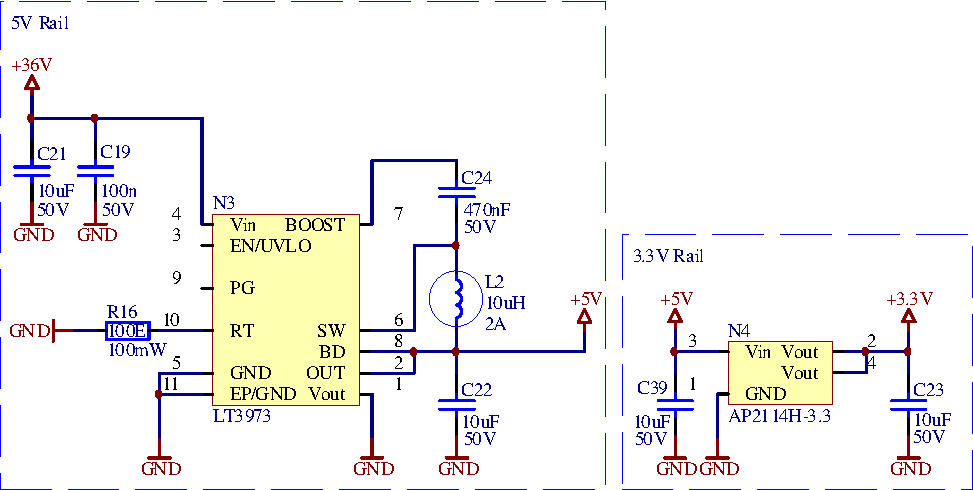
\includegraphics[width=.67\textwidth]{images/circuit/5v-3v-rails.pdf}
    %\caption{Speisung f\"ur 5V mittels Abwertswandler (links) und Speisung f\"ur 3.3V mittels Linearregler (rechts)}
    \caption{Supplying the \SI{5}{\volt} rail via switch-mode regulator (left) and the \SI{3.3}{\volt} rail via linear regulator (right)}
    \label{fig:circuit:rails}
\end{figure}


% **************************************************************************** %
\subsection{LT3741}
\label{subsec:lt3741}
% **************************************************************************** %

\emph{Note:} The schematic  for the  LT3471's circuit  is located  in appendix
\ref{appendix:lt3741:circuit} on page \pageref{appendix:lt3741:circuit}. It is
intended  to be  folded out  while reading  this section  of the  report. This
allows for convenient cross-referencing between  the circuit schematic and the
text without needing to insert multiple  copies of the schematic or constantly
scrolling back and forth through the report.

The most important reasons we chose  the LT3741 to regulate the output voltage
are as follows:

\begin{itemize}
    \item \textbf{Proven Technologies.}
        Switch-mode  regulators have  been around  for decades  and have  been
        perfected by many engineers.
    \item \textbf{Voltage and current requirements.}
        The device is specified to output voltage levels between \SI{0}{\volt}
        and  \SI{24}{\volt} and  current  levels  between \SI{0}{\ampere}  and
        \SI{3.5}{\ampere}.   Further, the  ripple voltage  is specified  to be
        $\le\SI{300}{\milli\volt}$  and the  ripple  current  is specified  to
        be  $\le\SI{100}{\milli\ampere}$. The  LT3741  fulfills all  of  these
        requirements.
    \item \textbf{The importance of power absorption.}
        Most switch-mode regulators are only  able to \emph{supply} power, but
        are  incapable of  \emph{absorbing} power. Because  our device  may be
        connected in series  (or parallel) with other power  supplies, it must
        have  the ability  to absorb  power  (which is  the case  if, it  were
        connected to a  voltage source outputting a higher  voltage level than
        our own).
    \item \textbf{Control inputs.}
        The LT3741  has dedicated  input control pins  to change  directly the
        output  current. This simplifies  the  design  because no  complicated
        additional circuitry is required.
\end{itemize}

%\begin{figure}[th!]
%    \center
%    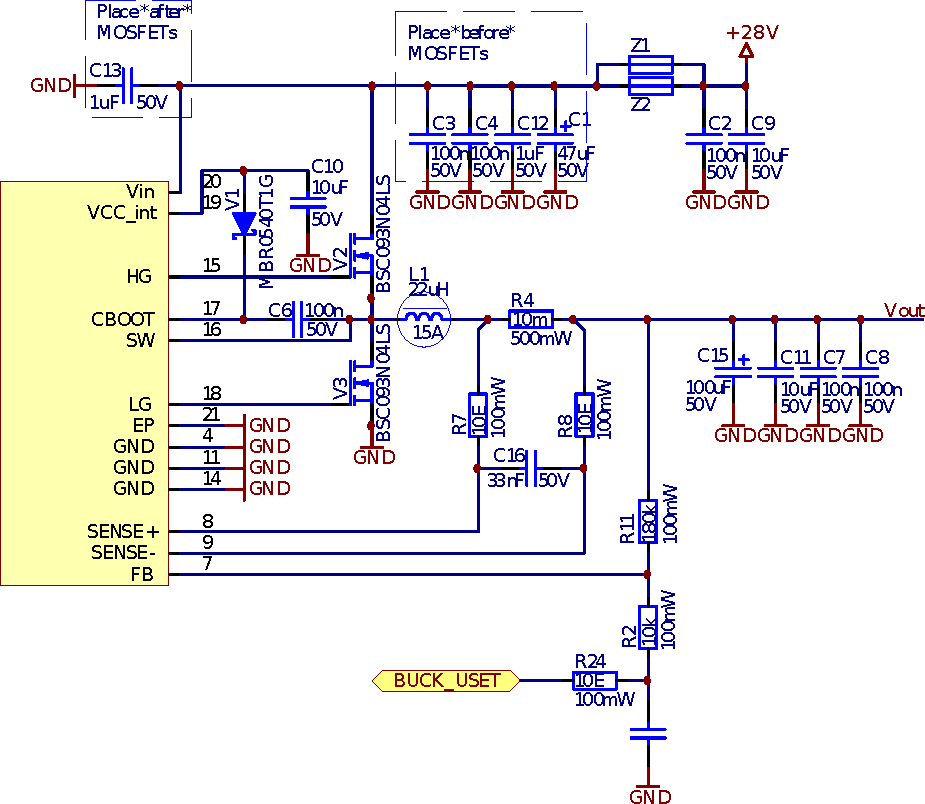
\includegraphics[width=.67\textwidth]{images/circuit/buck.pdf}
%    %\caption{Herzst\"uck des Projektes: Aufbau des LT3741 CVCC Synchronwandler}
%    \caption{The device's heart: Overview over circuit for the LT3741 CCVC synchronous converter.}
%    \label{fig:circuit:buck}
%\end{figure}

Figure \ref{fig:circuit:buck} on the fold-out (see \emph{Note} above) presents
an overview  for the LT3741's  circuit, parts of  which are discussed  in more
detail in  the following paragraphs:  Bypass  capacitors, switching frequency,
inductors, MOSFETs and measuring output current and output voltage.


% **************************************************************************** %
\subsubsection{Bypass Capacitors}
% **************************************************************************** %

The LT3741 is powered by the \SI{28}{\volt}  rail, which can be seen in Figure
\ref{fig:circuit:buck} in the  top right. The switching of  the MOSFETs causes
the LT13741  to consume high amounts  of power in short  bursts. This leads to
the LT3741  feeding high  frequency disturbance  back into  the \SI{28}{\volt}
rail, which  could lead  to disturbances  in the  rest of  the circuit  if not
handled correctly.  As a countermeasure,  a multitude of different ceramic and
electrolytic bypass  capacitors in parallel  are used.  Additionally,  we used
ferrite beads, placed  in series with the supply to  absorb any high frequency
feedback.


% **************************************************************************** %
\subsubsection{Switching Frequency}
% **************************************************************************** %

There is a trade-off when  selecting the switching frequency $f_S$. The higher
$f_S$,  the lower  the output  ripple voltage  will be. However,  the LT3741's
power  consumption will  also increase  due to  switching losses.   Generally,
$f_S$ is to be maximised to reduce ripple.

Because so  much depends  on $f_S$,  it is more  convenient to  determine this
value empirically through simulations. The  most suitable value was determined
to be $f_S \approx\SI{800}{\kilo\hertz}$. In the remaining calculations, $f_S$
is assumed to be \SI{1}{\mega\hertz} to allow for some leeway.

%A specific  resistor on one  of the LT3741's inputs  is used to  configure the
%switching frequency $f_S$.


% **************************************************************************** %
\subsubsection{Inductor Selection}
\label{subsubsec:lt3741:inductors}
% **************************************************************************** %

The   size    of   the    inductor   $L_1$,    as   illustrated    in   Figure
\ref{fig:circuit:buck}  on  the fold-out,  was  calculated  using the  formula
below:

\begin{equation}
    L_1 = \left( \frac{V_{in} \cdot V_{out} - V_{out}^2}{0.3 \cdot f_S \cdot I_O \cdot V_{in}} \right) = \SI{6}{\micro\henry}
    \label{eq:circuit:buck:inductor}
\end{equation}

where  $V_{in}$ equals  the  input voltage  \SI{28}{\volt},  $V_{out}$ is  the
output voltage  at peak  power (which exists  at $V_{out}  = \SI{14}{\volt}$),
$f_S$ is the switching frequency  \SI{1}{\mega\hertz} and $I_O$ is the maximum
output  current, assumed  to be  $I_O  = \SI{5}{\ampere}$,  allowing for  some
additional leeway.   A larger  inductor of  $L_1 =  \SI{22}{\micro\henry}$ was
selected to further decrease ripple current.

In addition to the inductance, the maximum current rating, DCR, and saturation
current are also important factors to consider. The inductor's peak current is
calculated using
\begin{equation}
    I_{L_{1_{peak}}} = I_O + \left( \frac{V_{in} \cdot V_{out} - V_{out}^2}{2 \cdot f_S \cdot L_1 \cdot V_{in}} \right) = \SI{5.2}{\ampere}
    \label{eq:circuit:buck:inductor_peak}
\end{equation}

Where  $V_{in}$ equals  the  input voltage  \SI{28}{\volt},  $V_{out}$ is  the
output voltage  at peak  power (which exists  at $V_{out}  = \SI{14}{\volt}$),
$f_S$ is  the switching frequency  \SI{1}{\mega\hertz}, $L_1$ is the  value of
the selected inductor (\SI{22}{\micro\henry}) and  $I_O$ is the maximum output
current, assumed  to be  $I_O =  \SI{5}{\ampere}$.  The  inductor's saturation
current  was  sized  $1.2$  times  higher than  the  peak  current. With  this
defined,  a list  of  possible inductors  could be  compiled,  shown in  Table
\ref{tab:circuit:buck:inductor} in  appendix \ref{appendix:inductors}  on page
\pageref{appendix:inductors}.   We chose  the \emph{732-4237-1-ND}  because it
has the lowest DCR (direct current resistance) of the models listed.


% **************************************************************************** %
\subsubsection{MOSFET Selection}
\label{subsubsec:lt3741:mosfets}
% **************************************************************************** %

In contrast to a non-synchronous  regulator, our design uses two complementary
MOSFETs $V_2$ and $V_3$ (in the middle of Figure \ref{fig:circuit:buck} on the
fold-out) , whereby $V_3$ acts as  an active replacement for the free wheeling
diode  typically found  in  non-synchronous designs. As  mentioned earlier,  a
crucial feature of  this device is the ability to  \emph{absorb} power.  $V_3$
does this by regulating current in the opposite direction through the inductor
$L_1$.

When  selecting  switching  MOSFETs,  the  following  parameters are critical in
determining the best devices for a given application: $Q_G$ (Total Gate Charge),
$R_{DS_{(on)}}$ (On-Resistance), $Q_{GD}$ (Gate to Drain Charge), $Q_{GS}$ (Gate
to Source  Charge),  $R_G$ (Gate Resistance), $V_{GS}$ (gate-to-source voltage),
$V_{DS}$  (drain-to-source-voltage),  $I_{D_{max}}$  (peak  drain  current)  and
$V_{GS_{THR}}$ (gate threshold voltage).

The     maximum     drain     current     is     equal     to     the     peak
inductor    current    $I_{L_{1_{peak}}}$    as   calculated    in    equation
\ref{eq:circuit:buck:inductor_peak}: $I_{D_{max}}    =   I_{L_{1_{peak}}}    =
\SI{5.2}{\ampere}$

%\begin{equation}
%    I_{D_{max}} = I_{L_{1_{peak}}} = I_O + \left(\frac{V_{in}\cdot V_{out} - V_{out}^2}{2\cdot f_S \cdot L_1 \cdot V_{in}}\right) = \SI{5.2}{\ampere}
%    \label{eq:circuit:buck:mosfet_id}
%\end{equation}

The maximum  drain-to-source voltage $V_{DS}$  must be greater than  the input
voltage  $V_{in}  =  \SI{28}{\volt}$,  including  transients,   otherwise  the
MOSFETs will be damaged. MOSFETs with $V_{DS} = \SI{40}{\volt}$ were therefore
selected.

The  signals driving  the  gates of  the  MOSFETs have  a  maximum voltage  of
\SI{5}{\volt}  with  respect to  the  source.   During start-up  and  recovery
conditions, the gate drive signals  may be as low as \SI{3}{\volt}. Therefore,
to  ensure that  the  LT3741  recovers properly,  the  maximum gate  threshold
voltage should  be less than  \SI{2}{\volt}. For a robust design,  the maximum
gate-to-source voltage $V_{GS}$ should be greater than \SI{7}{\volt}.

Power losses in  the MOSFETs are related to  the on-resistance $R_{DS{(on)}}$,
the  transition losses  related to  the gate  resistance $R_G$,  gate-to-drain
capacitance  $Q_{GD}$  and  gate-to-source  capacitance  $Q_{GS}$. Power  loss
to  the  on-resistance  is  an  Ohmic  loss,  $I^2  R_{DS_{(on)}}$. The  power
loss  in  the  high  side  MOSFET $V_2$  can  be  approximated  with  equation
\ref{eq:circuit:buck:mosfet_ploss}.

\begin{multline}
    P_{LOSS} = (\textrm{ohmic loss}) + (\textrm{transission loss}) \\
             \approx \left( I_O^2 \cdot R_{DS_{(on)}} \cdot \rho_T \right)
                    + \left( \frac{V_{in} \cdot I_O}{\SI{5}{\volt}} \cdot \left(Q_{GD} + Q_{GS} \right) \cdot \left( 2 \cdot R_G + R_{PU} + R_{PD} \right) \cdot f_S \right) \\
    \label{eq:circuit:buck:mosfet_ploss}
\end{multline}
whereby   $\rho_T$   is  a   temperature-dependant   term   of  the   MOSFET's
on-resistance.  Using \SI{70}{\degree C} as the maximum operating temperature,
$\rho_T$  roughly equals  $1.3$.  $R_{PD}$  and $R_{PU}$  are the  LT3741 high
side  gate  driver  output   impedances,  \SI{1.3}{\ohm}  and  \SI{2.3}{\ohm},
respectively.

Driving the gates also causes power loss in switching MOSFETs.  The total gate
charge, $Q_G$, must be charged and discharged switch each switching cycle. The
power is  lost to the internal  LDO within the  LT3741. The power lost  to the
charging of the gates is:
\begin{equation}
    P_{LOSS\_LDO} \approx \left( (V_{in} - \SI{5}{\volt} \right) \cdot \left( Q_{GLG} + Q_{GHG} \right) \cdot f_S
    \label{eq:circuit:buck:switching_loss}
\end{equation}
whereby $G_{GLG}$ is the  low side gate charge and $Q_{GHG}$  is the high side
gate charge.

Table  \ref{tab:circuit:buck:mosfet}  in  appendix  \ref{appendix:mosfets}  on
page  \pageref{appendix:mosfets} lists  possible MOSFETs  that meet  the above
constraints.  For  each one  the power  losses $P_{LOSS}$  and $P_{LOSS\_LDO}$
were calculated. The  MOSFET which  ended up  being selected  is not  the best
model, but it is a lot cheaper than the best fit and has better documentation.


% **************************************************************************** %
\subsubsection{Measurement of Output Voltage and Output Current}
\label{subsubsec:lt3741:feedback}
% **************************************************************************** %

\begin{minipage}{0.5\textwidth}
    The LT3741  is both voltage  regulated and current  regulated. The voltage
    divider  $R_{11}  \parallel  R_2$  (Figure  \ref{fig:circuit:buck:uset}  )
    allows for  the measurement of  the output  voltage, and a  shunt resistor
    $R_4$ allows  for the exact monitoring  of the current going  through coil
    $L_1$. The value  for resistor $R_4$ (fold-out  overview schematic, Figure
    \ref{fig:circuit:buck}) was chosen so that the maximum outoing current can
    be \SI{5}{\ampere}.

    Monitoring the  current is extremely  important for  a setup in  which the
    outgoing  voltage can  be constantly  changing. It allows  to predict  the
    behavior  of  the output  voltage,  thus  enabling  the device  to  better
    suppress spikes in  output voltage and spikes in the  current through coil
    $L_1$ (Figure \ref{fig:circuit:buck} on fold-out).

    Furthermore,  a  controller   regulated  by  current  can   also  be  used
    as  a  constant  current  source. This  property  is  of  importance  when
    the  operating  point   is  in  the  steeper  part  of   the  PV  module's
    I-V-curve  (where   small  changes   in  voltage   can  lead   to  drastic
    changes  in current,  see section  \ref{subsec:regimplementation} on  page
    \pageref{subsec:regimplementation}).

\end{minipage}
\begin{minipage}{0.5\textwidth}
    \center
    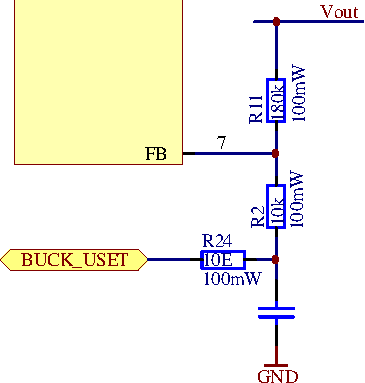
\includegraphics[width=.85\textwidth]{images/circuit/buck-uset.pdf}
    %\captionof{figure}{Regulation of output voltage by changing the reference voltage in the feedback loop via an analog reference voltage between \SI{0}{\volt} and \SI{1.21}{\volt}}
    \captionof{figure}{Circuit for regulating output voltage by changing reference voltage via $BUCK\_USET$ from the first DAC}
    \label{fig:circuit:buck:uset}
\end{minipage}

\begin{minipage}{.4\textwidth}
    The  values for  the feedback  resistors  $R_2$ and  $R_{11}$ were  chosen
    according to formula  \ref{eq:circuit:buck:feedback_resistors} so that the
    output voltage does not exceed \SI{23}{\volt}.
\end{minipage}
\begin{minipage}{.6\textwidth}
    \begin{equation}
        V_{out} = \SI{1.21}{\volt} \left( 1 + \frac{R_{11}}{R_2} \right)
        \label{eq:circuit:buck:feedback_resistors}
    \end{equation}
\end{minipage}

\begin{minipage}{.40\textwidth}
    By  increasing  $BUCK\_USET$  in formula  \ref{eq:circuit:buck:uset},  the
    outgoing  voltage can  then be  modified as  needed.  $BUCK\_USET$  is the
    analog voltage  coming from the  first DAC. The associated circuit  can be
    found in Figure \ref{fig:circuit:buck:uset}.
\end{minipage}
\begin{minipage}{.60\textwidth}
    \begin{equation}
        V_{out} = (\SI{1.21}{\volt} - BUCK\_USET) \cdot \frac{R_{11} + R_2}{R_2}
        \label{eq:circuit:buck:uset}
    \end{equation}
\end{minipage}


\begin{minipage}{.50\textwidth}
    In a manner analogous to regulating the output voltage, the maximum output
    current can  also be  controlled.  By applying  an analog  voltage between
    \SI{0}{\volt}  and \SI{1.5}{\volt}  at  input \code{CTRL1}  of the  LT3741
    controller,  the maximum  average  current going  through  coil $L_1$  and
    therefore the maximum output current can be directly controlled.

    The     corresponding    circuit     can     be     found    in     Figure
    \ref{fig:circuit:buck:iset}.  The maximum average  output current $I_o$ is
    calculated using equation \ref{eq:circuit:buck:output_current}.

    For  this, $V_{CTRL1}$  is the  analog reference  voltage coming  from the
    second DAC and  $R_4$ is the shunt  resistor (\SI{10}{\milli\ohm}, visible
    on the fold-out in Figure \ref{fig:circuit:buck}).

\end{minipage}
\begin{minipage}{.50\textwidth}
    \center
    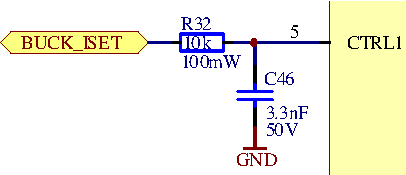
\includegraphics[width=.9\textwidth]{images/circuit/buck-iset.pdf}
    \captionof{figure}{Setting the maximum output current via reference voltage between \SI{0}{\volt} and \SI{1.5}{\volt}}
    \label{fig:circuit:buck:iset}
    \begin{equation}
        I_o = \frac{V_{CTRL1}}{30 \cdot R_4}
        \label{eq:circuit:buck:output_current}
    \end{equation}
\end{minipage}


\begin{minipage}{.50\textwidth}
    For  the  microcontroller  to  generate  appropriate  reference  voltages,
    it  needs  to   measure  both  output  voltage   and  output  current. The
    output    voltage   is    measured    with   the    circuit   in    Figure
    \ref{fig:circuit:buck:umeas}. The  values   for  resistors   $R_{12}$  and
    $R_{15}$  are such  that  voltage  $BUCK\_UMEAS$ is  scaled  to the  range
    between \SI{0}{\volt} and \SI{1.5}{\volt}.

    The  output   current  is  measured  differentially   via  shunt  resistor
    $R_5$. The    corresponding   circuit    can    be    seeen   in    Figure
    \ref{fig:circuit:buck:imeas}.

\end{minipage}
\begin{minipage}{.50\textwidth}
    \center
    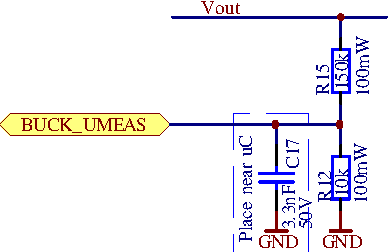
\includegraphics[width=.8\textwidth]{images/circuit/buck-umeas.pdf}
    \captionof{figure}{Measuring output voltage}
    \label{fig:circuit:buck:umeas}
\end{minipage}

\begin{figure}[th!]
    \center
    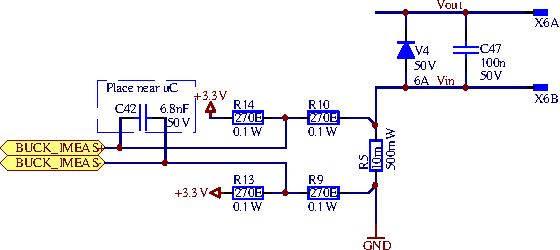
\includegraphics[width=.85\textwidth]{images/circuit/buck-imeas.pdf}
    \caption{Measuring output current}
    \label{fig:circuit:buck:imeas}
\end{figure}

\begin{minipage}{.50\textwidth}
A  particular problem  for this  measurement  is that  resistors $R_{10}$  and
$R_{14}$ cause a  bias current to flow through the  shunt resistor $R_5$, thus
leading  to an  offset $V_{offset}$  of the  measured voltage  over $R_5$,  as
calculated by equation \ref{eq:circuit:buck:shunt_offset}.
\end{minipage}
\begin{minipage}{.50\textwidth}
    \begin{equation}
        V_{offset} = \frac{ \SI{3.3}{\volt} \cdot R_5 }{ R_{14} + R_{10} + R_5 }
        \label{eq:circuit:buck:shunt_offset}
    \end{equation}
\end{minipage}

\begin{minipage}{.50\textwidth}
    Since  the  ADC  has  a  resolution   of  12  bits  and  a  reference  voltage
    of   \SI{3.3}{\volt},   one  voltage   increment   amounts   to  $V_{step}   =
    \frac{\SI{3.3}{\volt}}{2^{12}} = \SI{806}{\micro\volt}$

    Resistors $R_9$,  $R_{10}$, $R_{13}$  and $R_{14}$ should  be as  small as
    possible in order to reduce disturbances  in the traces, while at the same
    time being large enough for $V_{offset}$ to be smaller than $V_{step}$. In
    order for the ADC's holding time not to be too long (which happens roughly
    at $\geq \SI{5}{\kilo\ohm}$), they should however also not be too large.

    Thus, we can now  solve for the four resistor values,  as seen in on the right.
\end{minipage}
\begin{minipage}{.50\textwidth}

    %Equations \ref{eq:circuit:buck:shunt_offset} \ref{eq:circuit:buck:adc_step} can now
    %be solved for the four resistor values:

    \begin{align*}
                              V_{step} &\geq V_{offset} \\
        \frac{\SI{3.3}{\volt}}{2^{12}} &\geq \SI{3.3}{\volt} \cdot \frac{R_5}{R_x + R_5} \\
                      \frac{1}{2^{12}} &\geq \frac{R_5}{R_x + R_5} \\
                                   R_x &\geq \left( 2^{12} - 1 \right) \cdot R_5 \\
        \label{eq:solvethings}
    \end{align*}
    \hspace*{2em}whereby $\frac{R_x}{2} =  R_{9} = R_{10} = R_{13} =  R_{14}$.
\end{minipage}

This yields as its result $\frac{R_x}{2} \approx \SI{22}{\ohm}$.


\begin{minipage}{.50\textwidth}
    A  further  limitation,  especially  for  smaller  resistors,  is  not  to
    dissipate  too  much  power. For  this   reason,  the  resistors  will  be
    dimensioned  slightly   higher  at  \SI{270}{\ohm}. Thus,   the  resulting
    dissipated  power for  all  four resistors  is  calcualted using  equation
    \ref{eq:P_loss}.
\end{minipage}
\begin{minipage}{.50\textwidth}
    \begin{equation} \label{eq:P_loss}
        P_{loss} \approx \frac{\left(\SI{3.3}{\volt}\right)^2}{2\cdot \SI{270}{\ohm}} \approx \SI{20}{\milli\watt}
    \end{equation}
\end{minipage}

The measured  voltage at the  shunt resistor is comparatively  small. For this
reason, we use the microcontroller's integrated pre-amplifier (PGA), which can
attain a gain  of up to factor  64. The amplified signal is then  passed on to
the internal differential ADC.


% **************************************************************************** %
\subsubsection{Output}
% **************************************************************************** %

Two  banana  plugs  $X_{6A}$  and  $X_{6B}$  provide  the  connection  to  the
output  voltage,  while  reverse  voltage protection  is  achieved  via  diode
$V_4$.   (Figure \label{fig:circuit:output}).   An external  reference voltage
of  \SI{1.5}{\volt}  is  used to  ensure  that  the  ADCs  and DACs  can  make
accurate  measurements and  can  be used  over their  full  range (see  figure
\ref{fig:circuit:vref}).

\begin{minipage}{.50\textwidth}
    \center
    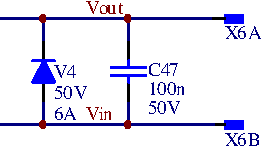
\includegraphics[width=.9\textwidth]{images/circuit/output-connectors.pdf}
    \captionof{figure}{Reverse voltage protection at output}
    \label{fig:circuit:output}
\end{minipage}
\begin{minipage}{.50\textwidth}
    \center
    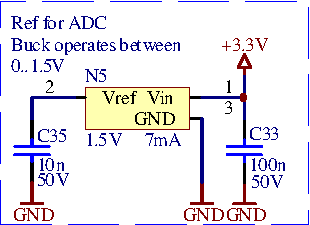
\includegraphics[width=.8\textwidth]{images/circuit/vref.pdf}
    \captionof{figure}{%
        \SI{1.5}{\volt} reference voltage for full-range operation of DACs
        and DACs
    }
    \label{fig:circuit:vref}
\end{minipage}



% **************************************************************************** %
\subsubsection{Enable and Under-Voltage Lockout circuit}
% **************************************************************************** %

\begin{minipage}{0.5\textwidth}
    The  LT3741's  \emph{Enable}   input  is  enabled  and   disabled  by  the
    microcontroller's $BUCK\_EN$ signal  on one hand, on the other  hand it is
    can  be  forcibly  disabled  in  hardware  when  the  \SI{28}{\volt}  rail
    drops below  \SI{25}{\volt}. This allows for a  controlled and predictable
    behavior of  the LT3741  during power-on and  power-off. The corresponding
    circuit can be found in Figure \ref{fig:circuit:uvlo}.

    In  case of  under-voltage, $N_6$  switches  on and  the transistor  $V_6$
    starts to  conduct, thus  pulling the  \emph{Enable} input  to \emph{Low}.
    Voltage $BUCK\_UVLO$ triggers an interrupt in the microcontroller.
\end{minipage}
\begin{minipage}{0.5\textwidth}
    \center
    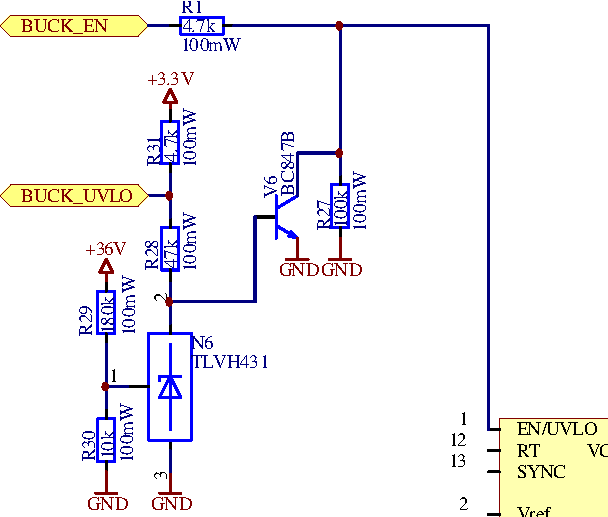
\includegraphics[width=.8\textwidth]{images/circuit/uvlo.pdf}
    \captionof{figure}{Under-Voltage Lock-Out (UVLO) allows for controlled power-on and power-off of the controller}
    \label{fig:circuit:uvlo}
\end{minipage}




% **************************************************************************** %
%\subsection{Push/Twist Button}
% **************************************************************************** %

%\begin{figure}[th!]
    \center
    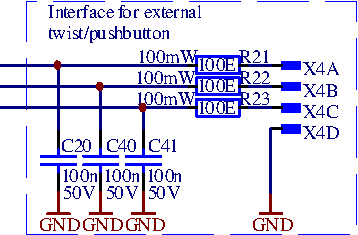
\includegraphics[width=.4\textwidth]{images/circuit/pushbutton.pdf}
    \caption{twist push button}
    \label{fig:circuit:pushbutton}
\end{figure}




% **************************************************************************** %
\clearpage
\section{PCB Design}
\label{sec:pcb}
% **************************************************************************** %
When designing  a PCB --  especially when a  switch-mode power converter  is a
central  component to  the  design --  the location  of  components and  their
routing (electrical connections) can be  critical for correct operation.  Some
of the more important items that were considered are listed here.
\begin{itemize}
    \item
        High frequency, high power loops are routed as tightly as possible.
    \item
        Sensitive, high impedance traces are kept separate from other signals
        and routed as differential pairs where necessary.
    \item
        Digital logic is kept separate from analog and high power circuitry.
    \item
        Power rails and their bypass capacitors need to be placed intelligently.
    \item
        Larger copper areas can be used to meet heat dissipation requirements.
    \item
        The positioning of mechanical parts can be annoying because they take up
        way more space than what one might initially, naively, expect.
\end{itemize}

\begin{minipage}{0.5\textwidth}
    Figure \ref{fig:pcb:partitioning}  shows how  our \SI{60x60}{\milli\meter}
    printed circuit board is partitioned. The ground plane has been split from
    top to  bottom, physically  separating partition  \emph{A} from  the other
    three partitions.  The LT3741 is placed in the centre where top and bottom
    planes join  because it must  communicate both  with the digital  logic as
    well  as  the  high  power  circuitry. Partition  \emph{A}  contains  high
    power/high frequency  components, such as  the two switching  MOSFETs, the
    inductor, and the output capacitors,  whereas the other partitions contain
    more  sensitive circuitry  (in particular  partition \emph{C}). The  split
    helps minimising crosstalk.

    Partition \emph{C}  contains the micro controller,  LCD header, push/twist
    button header and other digital components.

    Partition \emph{B} contains the  components responsible for generating the
    three voltage  rails discussed in section  \ref{sec:voltage_rails}. It was
    placed at  the bottom of  the board where the  power input is  located, to
    minimize the trace  lengths required for power distribution  on the board,
    and  it  was also  placed  far  away  from  partition \emph{B}  such  that
    interference with the digital circuitry is minimized.

    Partition \emph{D} is  electrically isolated from the rest  of the circuit
    and contains  the components  responsible for  USB communication.   It was
    isolated because  the voltage potential of  a connected USB device  may be
    different than the potential our device is running on.

    Figure  \ref{fig:pcb:loops1}  shows the  two  critical  loops where  short
    intervals  of high  amounts  of  current flow  in  this design. The  first
    (green) loop is  active when the switching MOSFET $V_2$  is conducting and
    transferring  charge  from  the  input  bypass  capacitors  $C_3$,  $C_4$,
    $C_{12}$ and $C_1$ through the resistor $R4$ into the inductor $L_1$.
\end{minipage}
\begin{minipage}{0.5\textwidth}
    \centering
    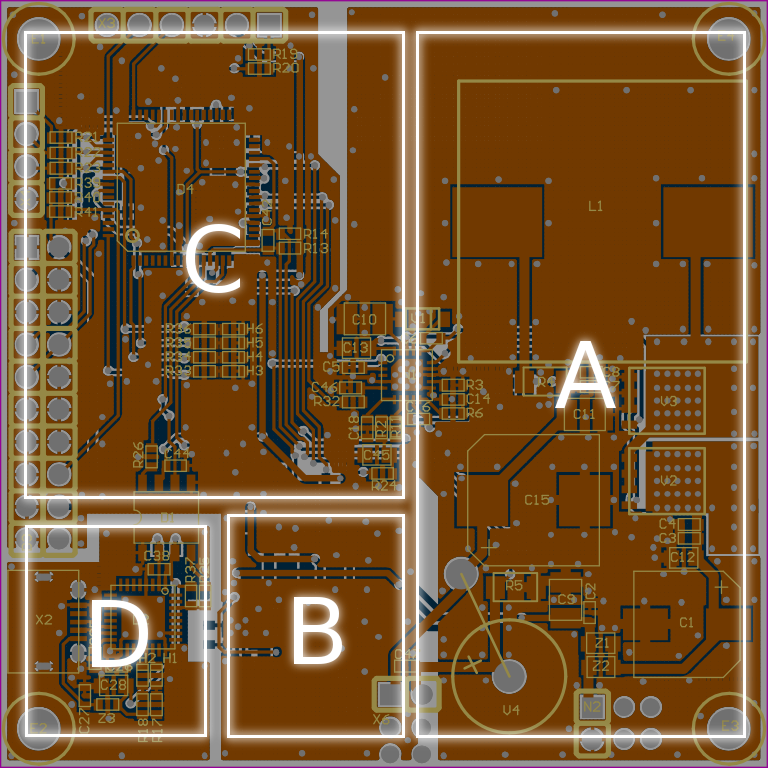
\includegraphics[width=.9\linewidth]{images/pcb/partitioning.png}
    \captionof{figure}{Partitioning scheme of component groups.
        \textbf{A:} High power components
        \textbf{B:} Voltage rails
        \textbf{C:} Digital logic
        \textbf{D:} Isolated transceiver logic
    }
    \label{fig:pcb:partitioning}
    \centering
    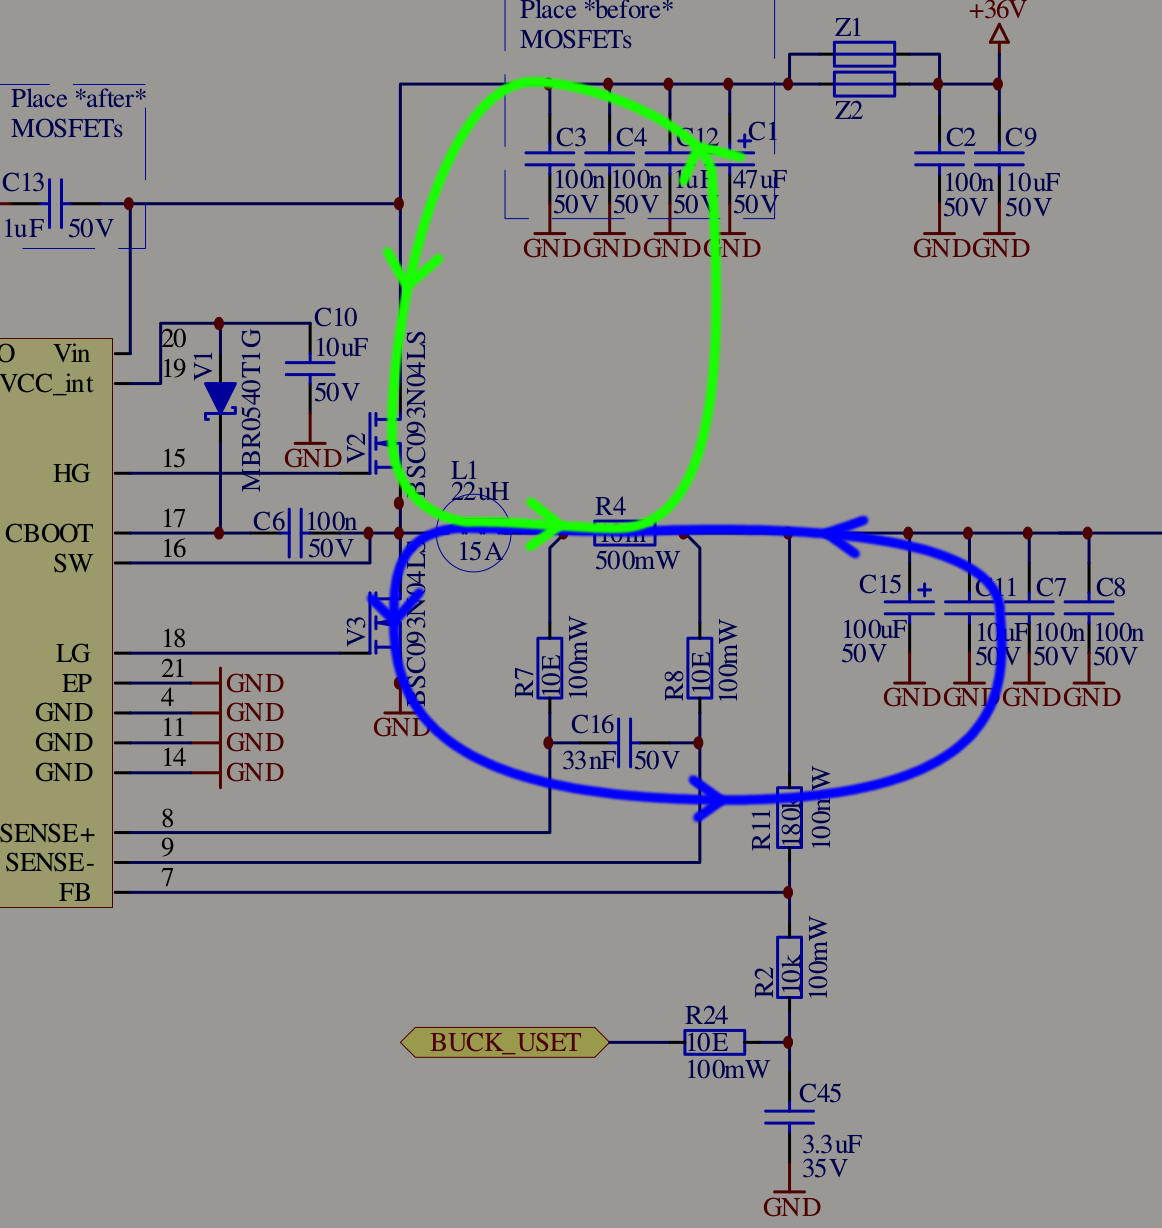
\includegraphics[width=.9\textwidth,trim=0 25mm 0 0,clip]{images/circuit/schematic_high_current.png}
    \captionof{figure}{Critical high current, high frequency loops in the schematic. Blue indicates the current path of the first critical loop, green the second.}
    \label{fig:pcb:loops1}
\end{minipage}

The second (blue) loop is active when the switching mosfet $V_3$ is conducting
and transferring  charge from  the inductor $L_1$  through the  resistor $R_4$
into the output bypass capacitors $C_{15}$, $C_{11}$, $C_7$ and $C_8$.




%\begin{figure}[h!]
%    \center
%    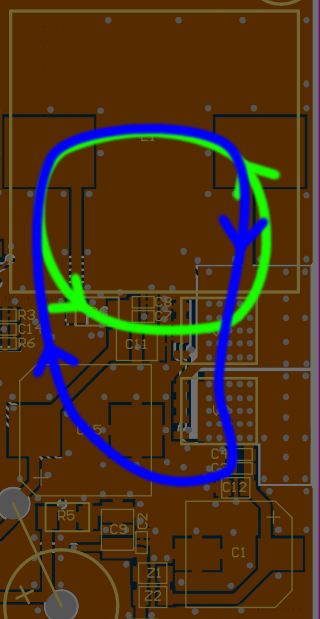
\includegraphics[width=.3\textwidth]{images/pcb/buck2.png}
%    \caption{High current, high frequency loops are routed as tightly as possible}
%    \label{fig:pcb:loops2}
%\end{figure}



% **************************************************************************** %
\clearpage
\section{Software}
\label{sec:software}
% **************************************************************************** %
The software  is split  into two  primary parts: The  firmware running  on the
device itself,  and the  front-end \emph{Smooth}, used  to interface  with the
device from a PC via USB.
\subsection{Firmware}
\label{subsec:firmware}
%\begin{itemize}
%    \item
%        Wie wird das mathematische Modell in Software implementiert?
%    \item
%        Wie wird die Kommunikation mit einem PC implementiert? (Protokoll)
%    \item
%        Event-System
%    \item
%        User-Interface am Ger\"at
%\end{itemize}


\subsubsection{Constraints for the uC programm}

The chosen  microcontroller dsPIC33ep  provides 16kB  of ROM  and 2kB  of RAM,
12bit resolution  in the ADC  and DAC and up  to 60 MIPS  computing power. The
anti-aliasing filter of  the ADC is set  to 5khz, which means that  we need to
sample with at least  \SI{10}{\kilo\hertz}. However the LT3741 regulator takes
about \SI{300}{\micro\second} to  adjust its output voltage --  3 times longer
than our  sample rate. To remedy this  we use Oversampling by  factor 4, which
has  the nice  benefits  of giving  us  an additional  bit  of resolution  and
making the anti-aliasing  filter simpler. The main routine  for the adjustment
of  the  regulator  should  not  use  more than  25\%  of  the  CPU  time  and
must  run every  \SI{400}{\micro\second},  so  it must  not  take longer  than
\SI{100}{\micro\second} or about 6000 Instructions to finish one calculation.


\subsubsection{I-V Curve and Operating Points}
\label{subsec:iv-curve-operating-points}

The  I-V  curve  from  \eqref{eq:I-V} is implemented using a fixed point  library
supplied by Microchip. Since this library also provides an exponential function,
the implementation is made straightforward.

To  find the  target  operating point,  we calculate  the  load resistance  by
dividing the voltage  on the output by  the current on the  output $R_{load} =
U_{is} /  I_{is}$. Then we draw the  load line $I =  f(U) = U /  R_{load}$ and
find  the intersection  with the  I-V  curve of  the model.   This process  is
pictured in Figure \ref{fig:model:approx}.  The intersection is found by using
a binary search algorithm, which is converging slower than newton's method but
more stable -- Newton's method can fail if $V_T$ in \eqref{eq:I-V} is small.

If we want to use multiple curves to model the staircase characteristic shown in
Figure \ref{fig:model:steps} we  need to determine which curve is applicable for
a given load. This process can be made less CPU intensive if we precalculate the
resistance-thresholds by finding the intersections between two curves.  There is
always exactly one intersection if  $V_{oc1} > V_{oc2}$ and $I_{sc1} < I_{sc2}$.

\begin{minipage}{0.5\textwidth}
	\center
    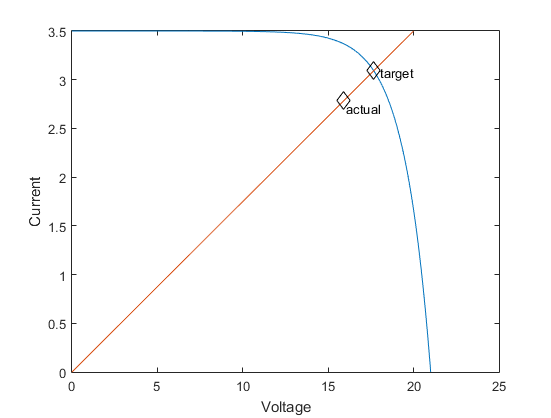
\includegraphics[width=.95\textwidth]{images/model/approx.png}
    \captionof{figure}{Actual and target operating points}
    \label{fig:model:approx}
\end{minipage}
\begin{minipage}{0.5\textwidth}
	\center
    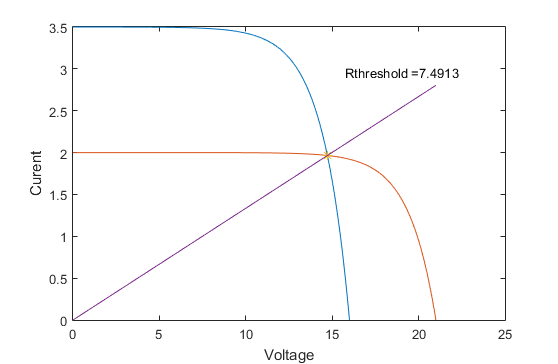
\includegraphics[width=.95\textwidth]{images/model/threshold.png}
    \captionof{figure}{Threshold resistance for selecting a curve}
    \label{fig:model:threshold}
\end{minipage}

\subsection{Front-End}
\label{subsec:frontend}
The  front-end  is  a software  tool  designed  to  provide  an easy  way  for
users to  model complicated  behaviours of photovoltaic  modules. The software
communicates with  the device via  a USB cable in  real time, which  means any
changes made  in the  tool have  an immediate effect  on the  generated output
voltage of the hardware device itself.

The front-end was built using the Qt framework\cite{ref:qt}, Qwt\cite{ref:qwt}
for 2D plots  and QwtPlot3D\cite{ref:qwtplot3d} for 3D plots,  and was written
in C++.  Qt was chosen because it  supports all major platforms and has a very
powerful set of  graphical components. Its Graphical User  Interface (GUI) can
be seen in  figure \ref{fig:front-end:screenshot}. On the left side  is a list
of  cells and  their  parameters. Cells can  be removed  or  added, and  their
individual  parameters  (open circuit  voltage,  short  circuit current,  dark
voltage  and  irradiation)  can  be  modified --  the  effects  of  which  are
immediate, as mentioned  above. A 2D plot shows what the  currently active I-V
characteristic curve looks like, along  with its corresponding power curve.  A
3D  plot  shows  the  behaviour  of  the  2D  power  curve  in  function  with
irradiation. In the  top right corner of  the GUI the actual  measured voltage
and current of the device is displayed.

\begin{figure}[th!]
    \centering
    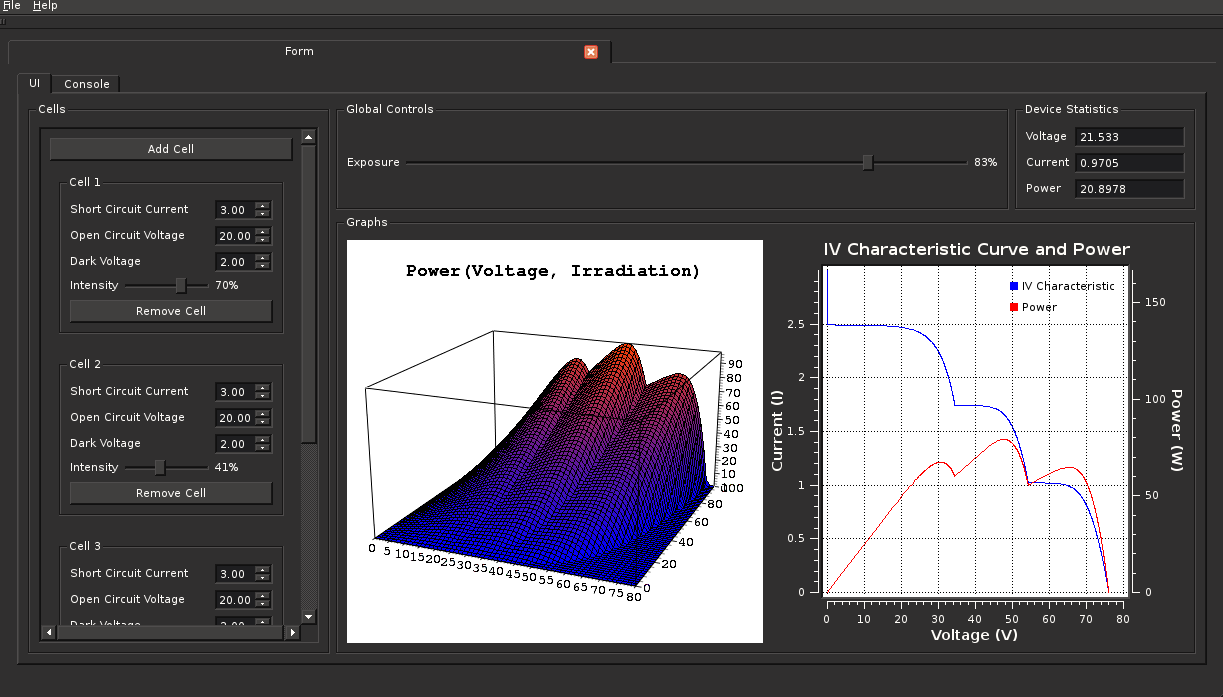
\includegraphics[width=.8\textwidth]{images/frontend/frontend.png}
    \caption{Screenshot of the front-end's Graphical User Interface (GUI)}
    \label{fig:front-end:screenshot}
\end{figure}

At this  point, the  front-end is  not yet  fully functional  as intended. The
graphical user  interface itself  is implemented  as planned,  but interfacing
with the  hardware lacks  yet a  few features. Partially,  this is  because we
could  not  test  all  its  functionality without  the  hardware  being  fully
operational. Another  reason  was  the   time  invested  into  diagnosing  the
issues related  to the buck converter  (section \ref{subsec:analysis_issue} on
pages  \pageref{subsec:analysis_issue}ff), which  needed to  be diverted  from
developing the front-end.

It is however in a solid proof-of-concept stage and ready to be finalised once
the device itself operates as intended.



% **************************************************************************** %
%\clearpage
\section{Verification}
\label{sec:verification}
% **************************************************************************** %
There are a variety of tests that can be conducted to verify the performance and
correctness of our  device.  The  following is a list of test fixtures and their
expected results based on simulations.

\subsection{Test Fixtures}

\subsubsection{Trivial and Non-Trivial I-V Curves}

Reproduction of a custom I-V  curve is tested by using the test fixture depicted
in Figure \ref{fig:verification:iv-circuit-fix}.

\begin{figure}[th!]
    \centering
    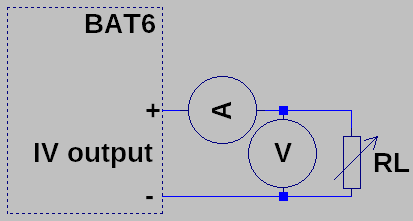
\includegraphics[width=.4\textwidth]{images/sim/iv-curve-circuit.png}
    \caption{Test fixture for measuring the device's IV characteristic curve}
    \label{fig:verification:iv-circuit-fix}
\end{figure}

The  voltage  and  current  is  measured  using  different resistive loads. This
measurement is performed twice using two different I-V curve configurations; one
``simple''  curve (using a single-cell  model)  and  one  ``complicated''  curve
(using a  multi-cell  model  where  some of the cells are shaded). The resulting
measurements are then compared with  the  theoretical  curves  seen  in  Figures
\ref{fig:verification:iv-simple}  and  \ref{fig:verification:iv-complicated} and
thus the device's accuracy can be evaluated.

\begin{figure}[th!]
    \centering
    \begin{minipage}{.4\textwidth}
        \centering
        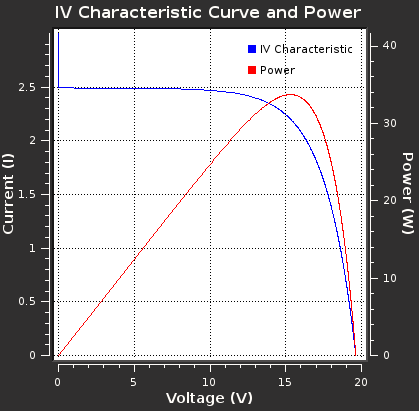
\includegraphics[width=.95\textwidth]{images/sim/iv-simple.png}
        \caption{Current/voltage characteristic curve (blue) and power/voltage characteristic curve (red) of a single-cell solar panel}
        \label{fig:verification:iv-simple}
    \end{minipage}
    \begin{minipage}{.4\textwidth}
        \centering
        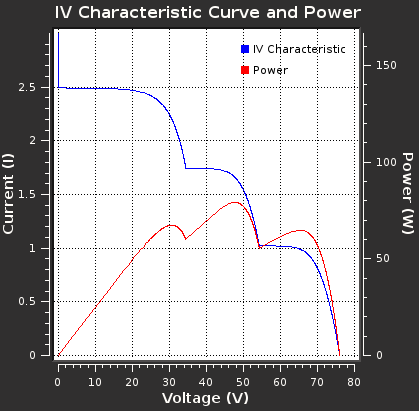
\includegraphics[width=.95\textwidth]{images/sim/iv-complicated.png}
        \caption{Current/voltage characteristic curve (blue) and power/voltage charactersticic curve (red) of a multi-cell solar panel, some cells are shaded, causing the staircase}
        \label{fig:verification:iv-complicated}
    \end{minipage}
\end{figure}

\subsubsection{Ripple Voltage and Ripple Current vs Resistive Load}

Using LTspice\cite{ref:ltspice}, the circuit  of  our  regulator was modeled and
the  peak-to-peak  ripple  current  and  voltage  was  simulated using different
resistive  loads ranging from \SI{100}{\milli\ohm} to  \SI{1}{\kilo\ohm}  at  an
output  voltage of \SI{12}{\volt}. Figure \ref{fig:verification:ripple_sim} is a
plot  of  the   ripple   current   and   voltage   versus  the  resistive  load.

\begin{figure}[th!]
    \centering
    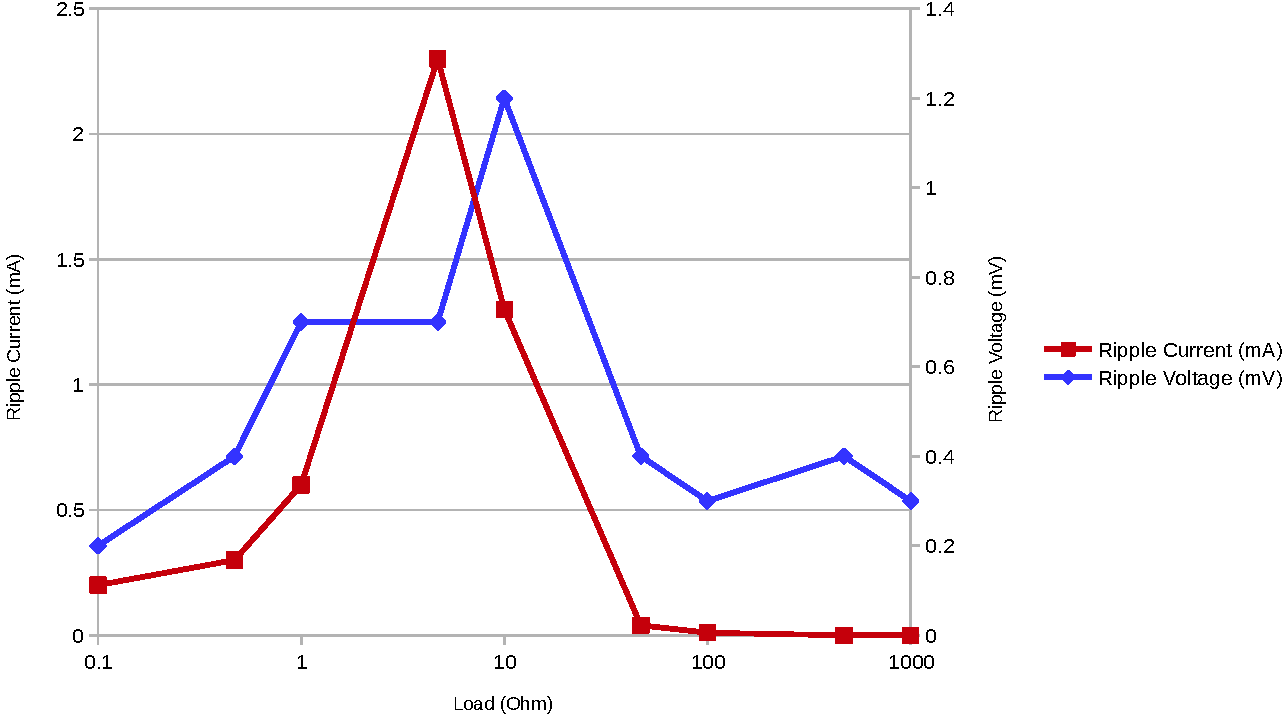
\includegraphics[width=.7\textwidth]{images/sim/ripple-vs-load.pdf}
    \caption{Simulation of the amplitude of the ripple voltage and ripple current vs different resistive loads, obtained using LTspice I-V's model of the LT3741}
    \label{fig:verification:ripple_sim}
\end{figure}

\begin{minipage}{0.5\textwidth}
    In  order   to  test  this   on  the   real  device,  a   constant  output
    voltage   of  \SI{12}{\volt}   is  programmed   and  a   potentiometer  is
    attached  to the  device's  output connectors,  as  illustrated in  Figure
    \ref{fig:verification:ripple_fix}

    The ripple  current is  measured over a  small sense  resistor $R_{sense}$
    using  an oscilloscope. The  ripple  voltage is  measured  using a  second
    channel of the oscilloscope by measuring the output voltage.
\end{minipage}
\begin{minipage}{0.5\textwidth}
    \centering
    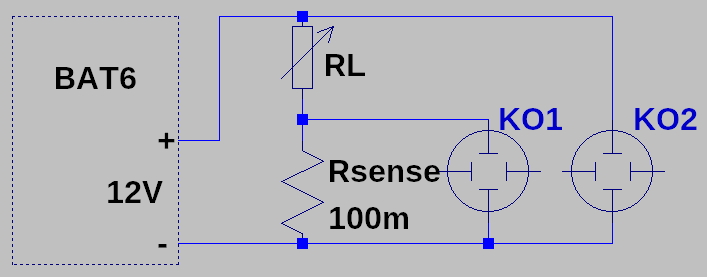
\includegraphics[width=.9\textwidth]{images/sim/ripple-fixture.png}
    \captionof{figure}{Test fixture for measuring ripple voltage \& ripple current of the device}
    \label{fig:verification:ripple_fix}
\end{minipage}

The peak-to-peak ripple voltage  and current is measured for different resistive
loads ranging from \SI{100}{\milli\ohm} to \SI{1}{\kilo\ohm} and compared to the
simulated model.

\subsubsection{Power Absorbtion}

\begin{minipage}{0.5\textwidth}
    As  stated  in  the  specifications,  the device  must  have  the  ability
    to  sink   current  as  well  as   source  current.   In  order   to  test
    this,  the   device  is  programmed   to  output  \SI{12}{\volt}   and  is
    connected  in  series  with  a  current limiting  resistor  and  a  second
    power  source  set   to  a  higher  voltage,  as   illustrated  in  Figure
    \ref{fig:verification:power_absorbtion_fix}.

    The second  voltage source is  slowly increased until  \SI{3}{\ampere} are
    flowing  through  the  current  limiting  resistor  $R_1$  (which  can  be
    determined by  measuring the  voltage over said  resistor), all  while the
    device's  output  voltage  is  closely monitored. The  output  voltage  is
    expected to remain constant.
\end{minipage}
\begin{minipage}{0.5\textwidth}
    \centering
    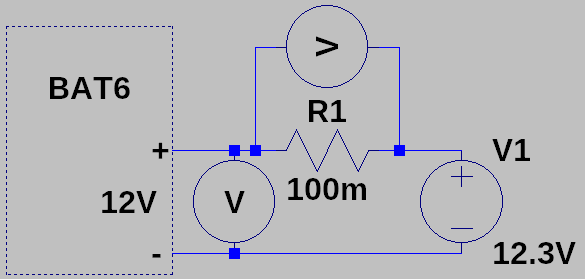
\includegraphics[width=.9\textwidth]{images/sim/power-absorbtion-fixture.png}
    \captionof{figure}{Test fixture for measuring power absorbtion of the device.}
    \label{fig:verification:power_absorbtion_fix}
\end{minipage}



\subsubsection{Transient Response}

\begin{minipage}{0.5\textwidth}
    This  test is  used  to  determine the  reaction  speed  of the  regulator
    and  the  I-V  control  algorithm   when  switching  quickly  between  two
    extreme  resistive  loads.    The  device  is  programmed   to  mimic  the
    behaviour  of  a simple  solar  panel  model.   As illustrated  in  Figure
    \ref{fig:verification:transient_fix} the output  voltage is measured using
    an oscilloscope and  various resistive loads are switched on  and off over
    the output using a MOSFET and a signal generator.
\end{minipage}
\begin{minipage}{0.5\textwidth}
    \centering
    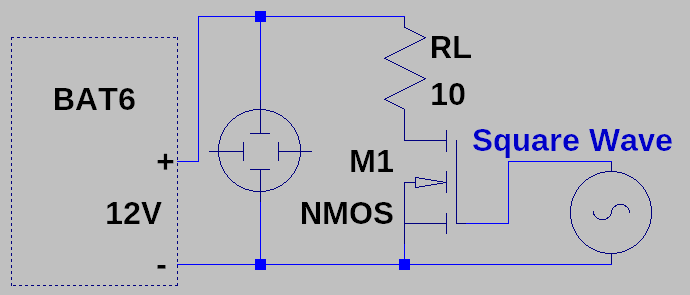
\includegraphics[width=.9\textwidth]{images/sim/transient-fixture.png}
    \captionof{figure}{Test fixture for measuring the transient response of the device}
    \label{fig:verification:transient_fix}
\end{minipage}

The frequency  of the signal  generator is  set to a  low value such  that the
device's output  voltage is  always stable  before the  load is  changed.  The
results of this  measurement will make a statement over  the propagation delay
of the  algorithm as well as  the time it  takes for the voltage  to stabilise
again.


\subsubsection{Reactive Loads}

In the coarse specification we  opted to test the device with various capacitive
and  inductive  loads  out  of  curiosity. During the course of the  project  we
learned that this is not an applicable test because reactive loads are primarily
used for testing the behaviour of power factor correction -- which, according to
the EN61000-3-2  regulations\cite{ref:pfc},  affect  devices consuming more than
\SI{75}{\watt},  meaning  that  the main power supply we use already implements
power factor correction and testing for this would  be meaningless. Furthermore,
the measurements we obtain  from  tests  using  reactive  loads would require an
immense  amount of additional research on our part before the results  could  be
interpreted in any  meaningful way. For this reason we have decided to omit this
test case.


\subsection{Measurement Results}

Unfortunately, we were unable to  operate the LT3741 for a period long enough to
conduct any of the measurements listed above.  The same regulator model (LT3741)
was  permanently  damaged  twice  in  a row. Please see the next section  for  a
detailed analysis on what we think the issue is and how we would proceed if more
time to do so were available.


\subsection{Analysis of the Issue}
\label{subsec:analysis_issue}

The  first regulator output the correct voltage  of  \SI{12}{\volt}  when  being
supplied  with  \SI{32}{\volt}.  Unplugging the device and re-plugging it into a
\SI{36}{\volt}  power  supply  instantly  damaged  it  permanently.  After  some
detailed measurements it  was  concluded  that  the  high-side driver inside the
LT3741  was somehow damaged and not operating as it should. Our  assumption  was
that -- since we were  operating  the device very closely to its maximum ratings
of  \SI{40}{\volt} -- during switching, the high-side MOSFET driver was  exposed
to transients exceeding the device's absolute maximum ratings  and thus damaging
the driver permanently.

The regulator was replaced  with a new one and the  supply voltage was lowered
from \SI{36}{\volt}  to \SI{28}{\volt} in  order to  give more leeway  for the
transient voltages. The new  regulator appeared to output  the correct voltage
of  \SI{12}{\volt}, so  a resistive  load  of \SI{80}{\ohm}  was connected  to
the  output of  the  regulator.  After  about  \SI{20}{\second} of  continuous
operation, the  output voltage  again dropped and  the device  was permanently
damaged. Unfortunately, we were  unable to capture some  vital measurements of
the transients  we were looking for  to confirm our suspicions  from the first
failure.  It is clear,  however, that the damage was not  caused by the device
overheating, as none  of the components were remotely warm  to the touch. This
seems to align with the transient theory.


\subsection{Simulating the Issue}

The physical  layout of the  regulator and the  MOSFETs is depicted  in Figure
\ref{fig:verification:long_traces_pcb}.   The  traces  connecting  the  Switch
(SW), High Gate (HG) and Low Gate  (LG) pins of the regulator to the switching
MOSFETs  are  fairly  long  (>\SI{2}{\centi\metre}). Most  of  the  time,  the
parasitic inductances and capacitances  are negligible. In this case, however,
it turned out that they are not.

The series  inductance  and  series  resistance  is  calculated using an on-line
calculator\cite{ref:trace_inductance}\cite{ref:trace_resistance}   (the   width,
length,    and    thickness    is    known   to    be    \SI{0.4}{\milli\metre},
\SI{2}{\centi\metre}  and \SI{35}{\micro\metre} respectively) and added  to  the
simulation   model  seen  in  Figure   \ref{fig:verification:long_traces_model}.

\begin{figure}[th!]
    \centering
    \begin{minipage}{.6\textwidth}
        \centering
        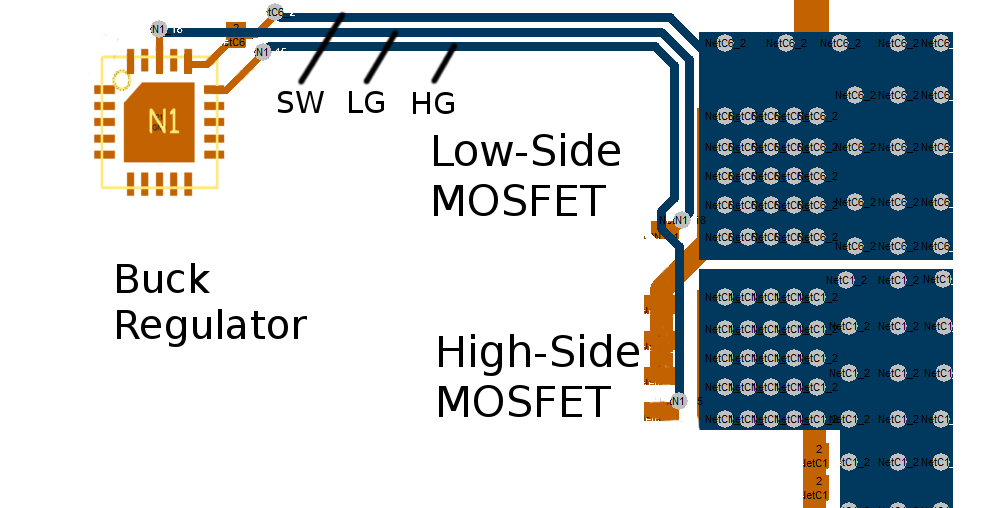
\includegraphics[width=.9\textwidth]{images/pcb/long-traces.png}
        \caption{Physical layout of MOSFETs and regulator}
        \label{fig:verification:long_traces_pcb}
    \end{minipage}
    \begin{minipage}{.38\textwidth}
        \centering
        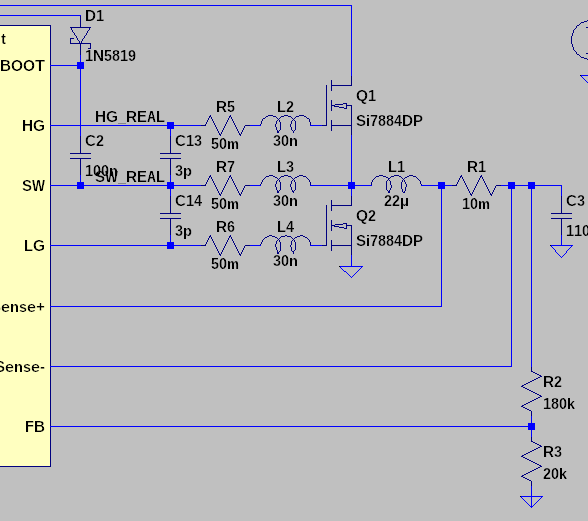
\includegraphics[width=.9\textwidth]{images/sim/lt3741-transients-circuit-real.png}
        \caption{Simulation model with long traces}
        \label{fig:verification:long_traces_model}
    \end{minipage}
\end{figure}

The voltage on the SW pin of the regulator  is  simulated  and  plotted.  Figure
\ref{fig:verification:long_traces_simulation}  compares  the   more   accurately
modelled curve (in blue, labelled \emph{sw\_real})  with  the ideal model of the
voltage on the SW pin (in yellow, labelled \emph{sw\_ideal}). The  two red lines
represent  the  expected  maximum  voltage  (\SI{28}{\volt})  and  the  device's
absolute maximum rating on the SW pin (\SI{40}{\volt}).

\begin{figure}[th!]
    \centering
    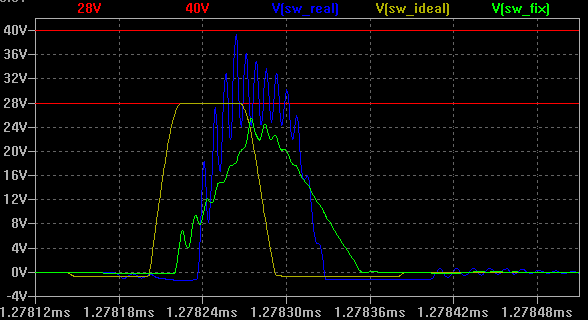
\includegraphics[width=.7\textwidth]{images/sim/lt3741-transients-sim.png}
    \caption{Simulation of voltage on SW pin. \emph{Yellow:} Idealised, \emph{blue:} actual, \emph{green}: actual, with series resistors as a fix.}
    \label{fig:verification:long_traces_simulation}
\end{figure}

It is clear that these small parasitic  inductances have a huge impact. The real
curve  (blue) exhibits ringing  with  an  amplitude  overshooting  the  expected
maximum voltage by  almost  \SI{12}{\volt}! It is therefore very likely that the
high driver was destroyed due to an over-voltage event.

The immediate solution to this problem  is  to add resistors in series with each
of  the  critical  connections  to  dampen  the  ringing.  The   effect   of   a
\SI{3.3}{\ohm} resistor in series  with  each  connection  is  plotted in figure
\ref{fig:verification:long_traces_simulation}     (green     curve,     labelled
\emph{sw\_fix}). When compared  to  the  ideal  and real curves, we see that the
peak voltage has been reduced to a much less dangerous level.

The more  optimal solution  (more elegant  and cheaper) is  to modify  the PCB
layout to drastically reduce the length of these traces.



% **************************************************************************** %
\clearpage
\section{Conclusions}
\label{sec:conclusion}
% **************************************************************************** %
The device is  assembled (as can be seein  in Figure \ref{fig:bat6:assembled})
and has  a functioning interface. Thanks  to our custom  PCB, we were  able to
make a very compact device (visible in Figure \ref{fig:bat6:internals}).  Most
sub circuits function  as intended (OLED, button, USB,  microchip), except for
the circuitry related to the buck  converter.  The front-end software has been
successfully brought to proof-of-concept stage  and is ready to be implemented
fully.

The  primary  thing   which  does  not  function  as  intended   is  the  buck
converter. We were however able to pinpoint  the likely cause of the issue and
are confident that  with more time and  a new hardware revision,  we could fix
this problem.

The next step would  now be to print a new PCB with  improvements based on our
simulations  from  section  \ref{sec:verification}  and  then  verify  correct
functionality of our device.

\begin{figure}[h!]
    \center
    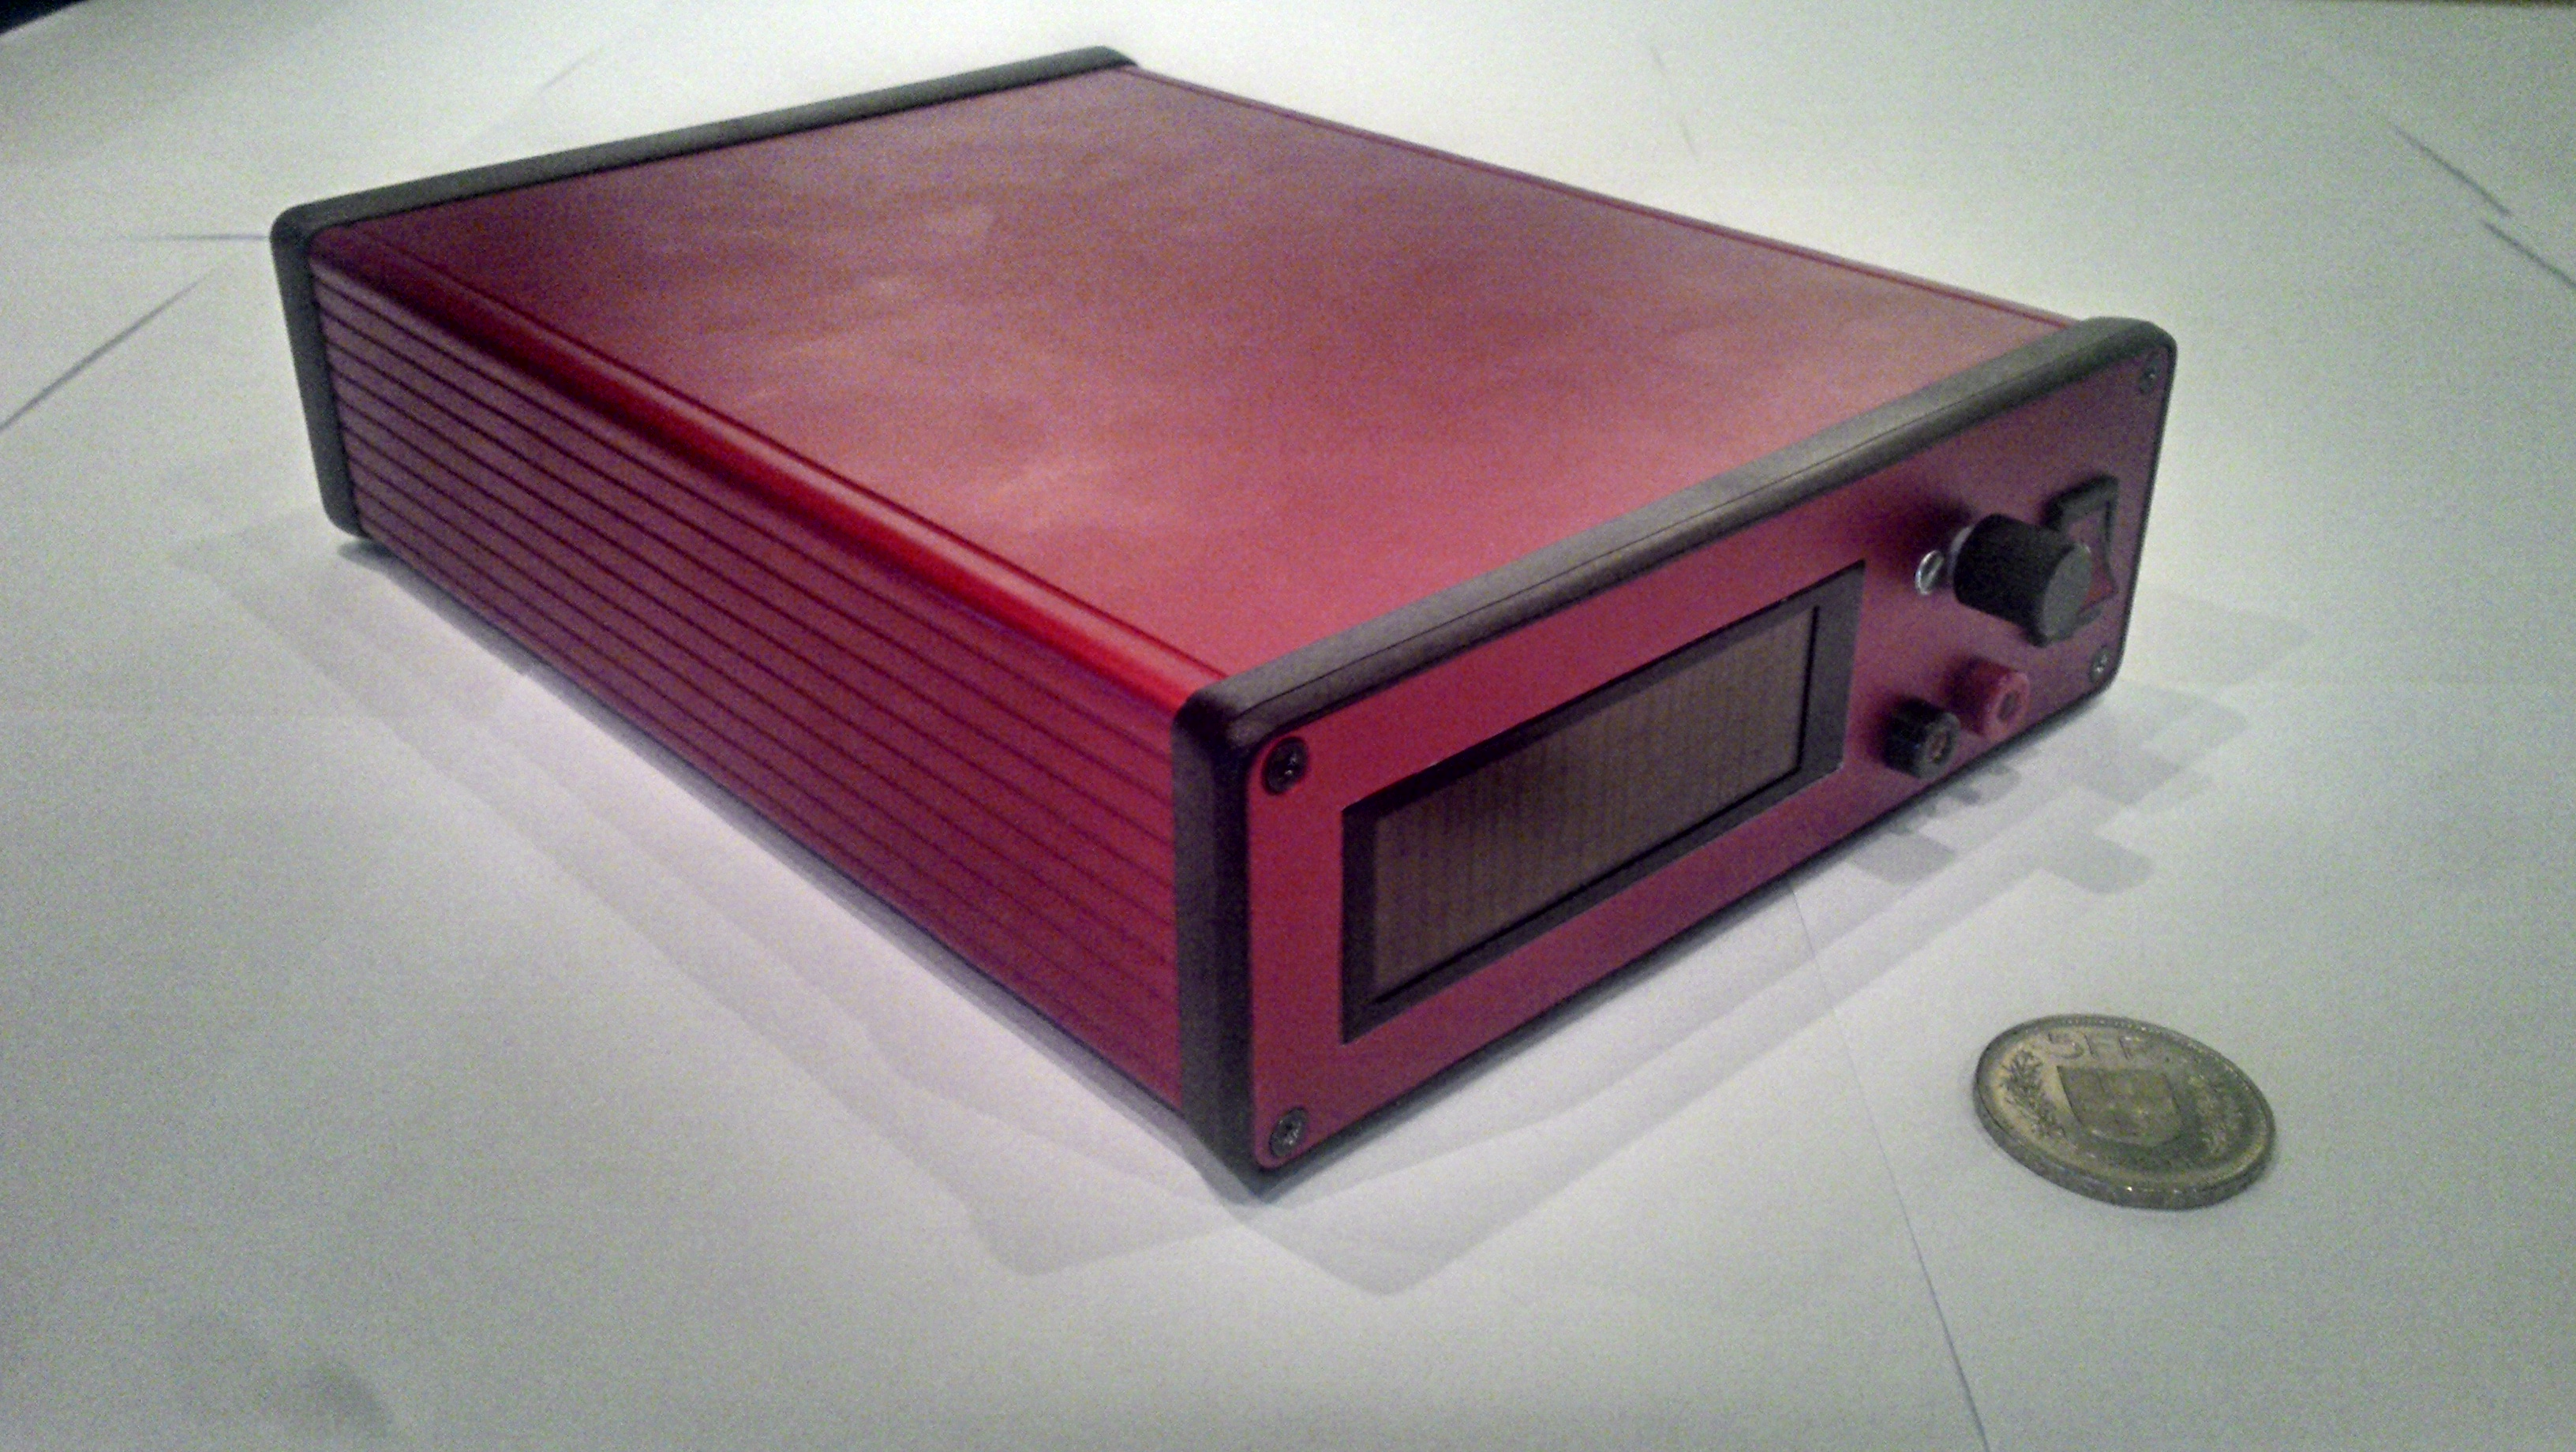
\includegraphics[width=.8\textwidth]{images/assembled.jpg}
    \caption{\emph{BAT6} assembled, 5 CHF coin for scale}
    \label{fig:bat6:assembled}
\end{figure}

\begin{figure}[h!]
    \center
    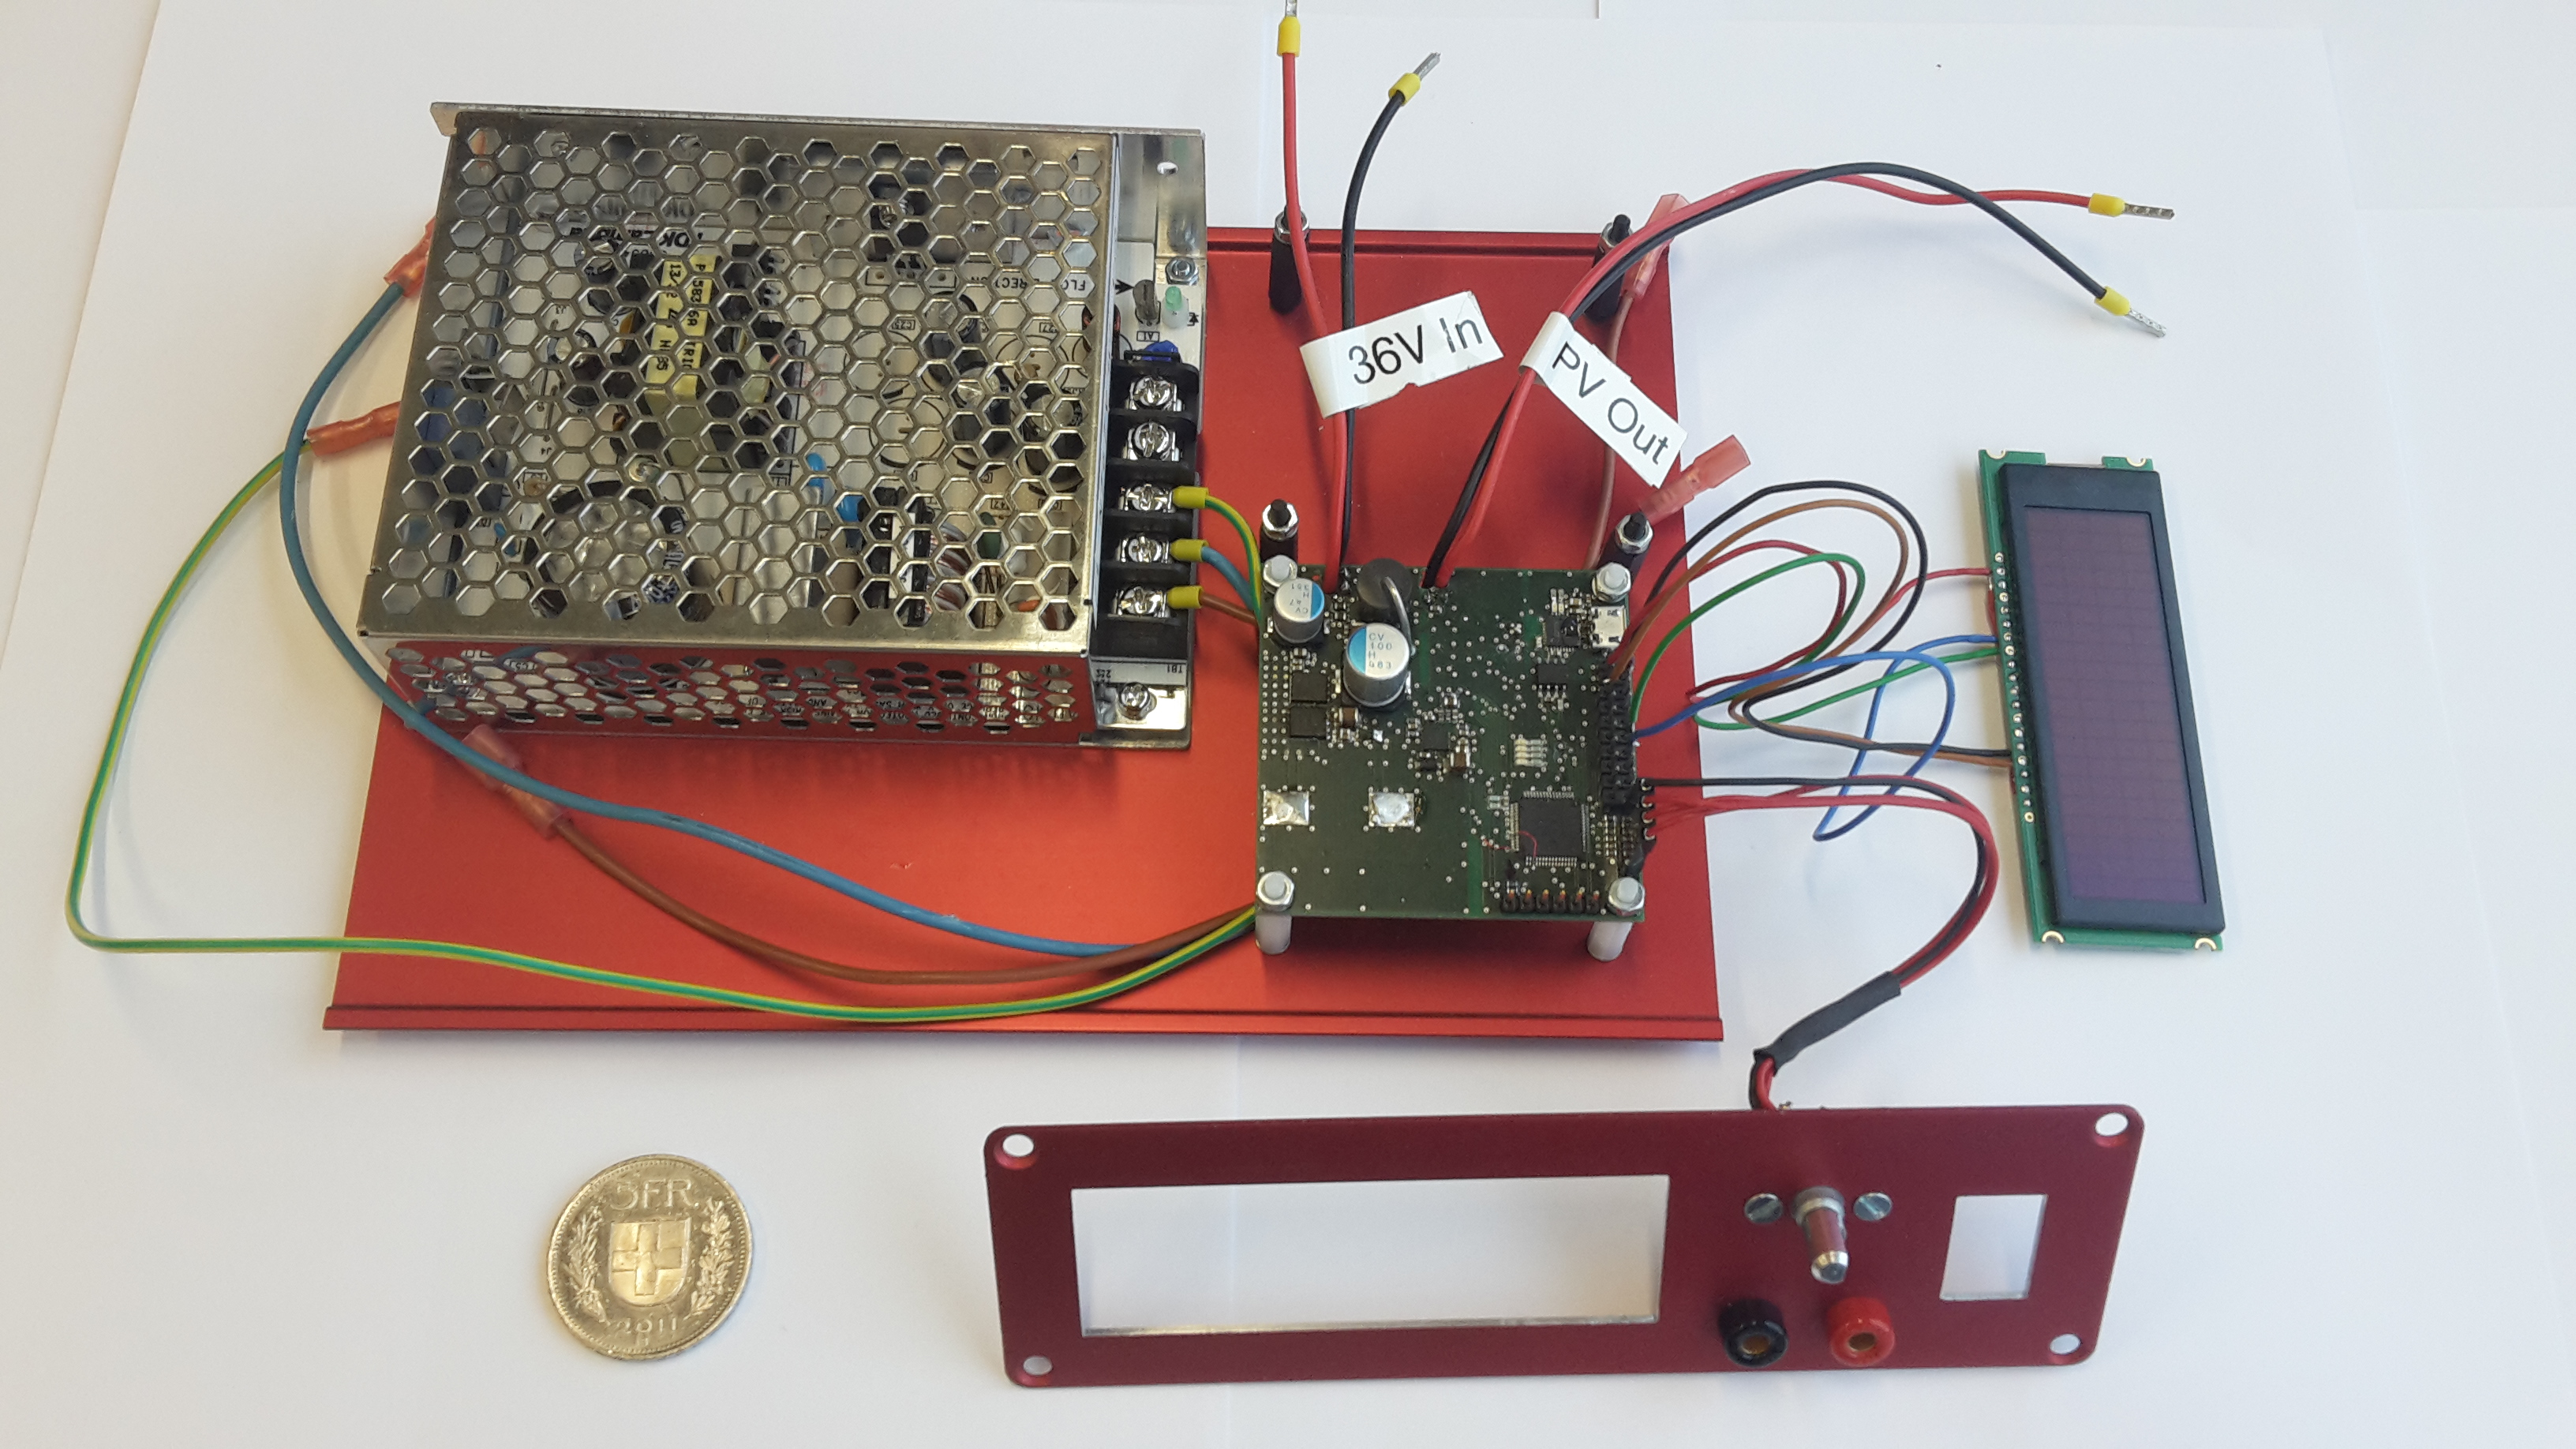
\includegraphics[width=.8\textwidth]{images/internals.jpg}
    \caption{\emph{BAT6}'s internals. Note the PCB's compact size. Most of the internal space is taken up by the power supply. 5 CHF coin for scale.}
    \label{fig:bat6:internals}
\end{figure}



% **************************************************************************** %
%\clearpage
%\section*{Unterschrift}
%\label{sec:signature}
% **************************************************************************** %
%\input{sections/signature.tex}


% **************************************************************************** %
\clearpage
\begin{appendices}
    %\appendixpage
    %\addappheadtotoc
    %\appendix
    %\section{Anhang}
    \label{sec:appendix}
    % ************************************************************************ %
    % **************************************************************************** %
\clearpage
\section{Specifications}
\label{appendix:specs}
% **************************************************************************** %

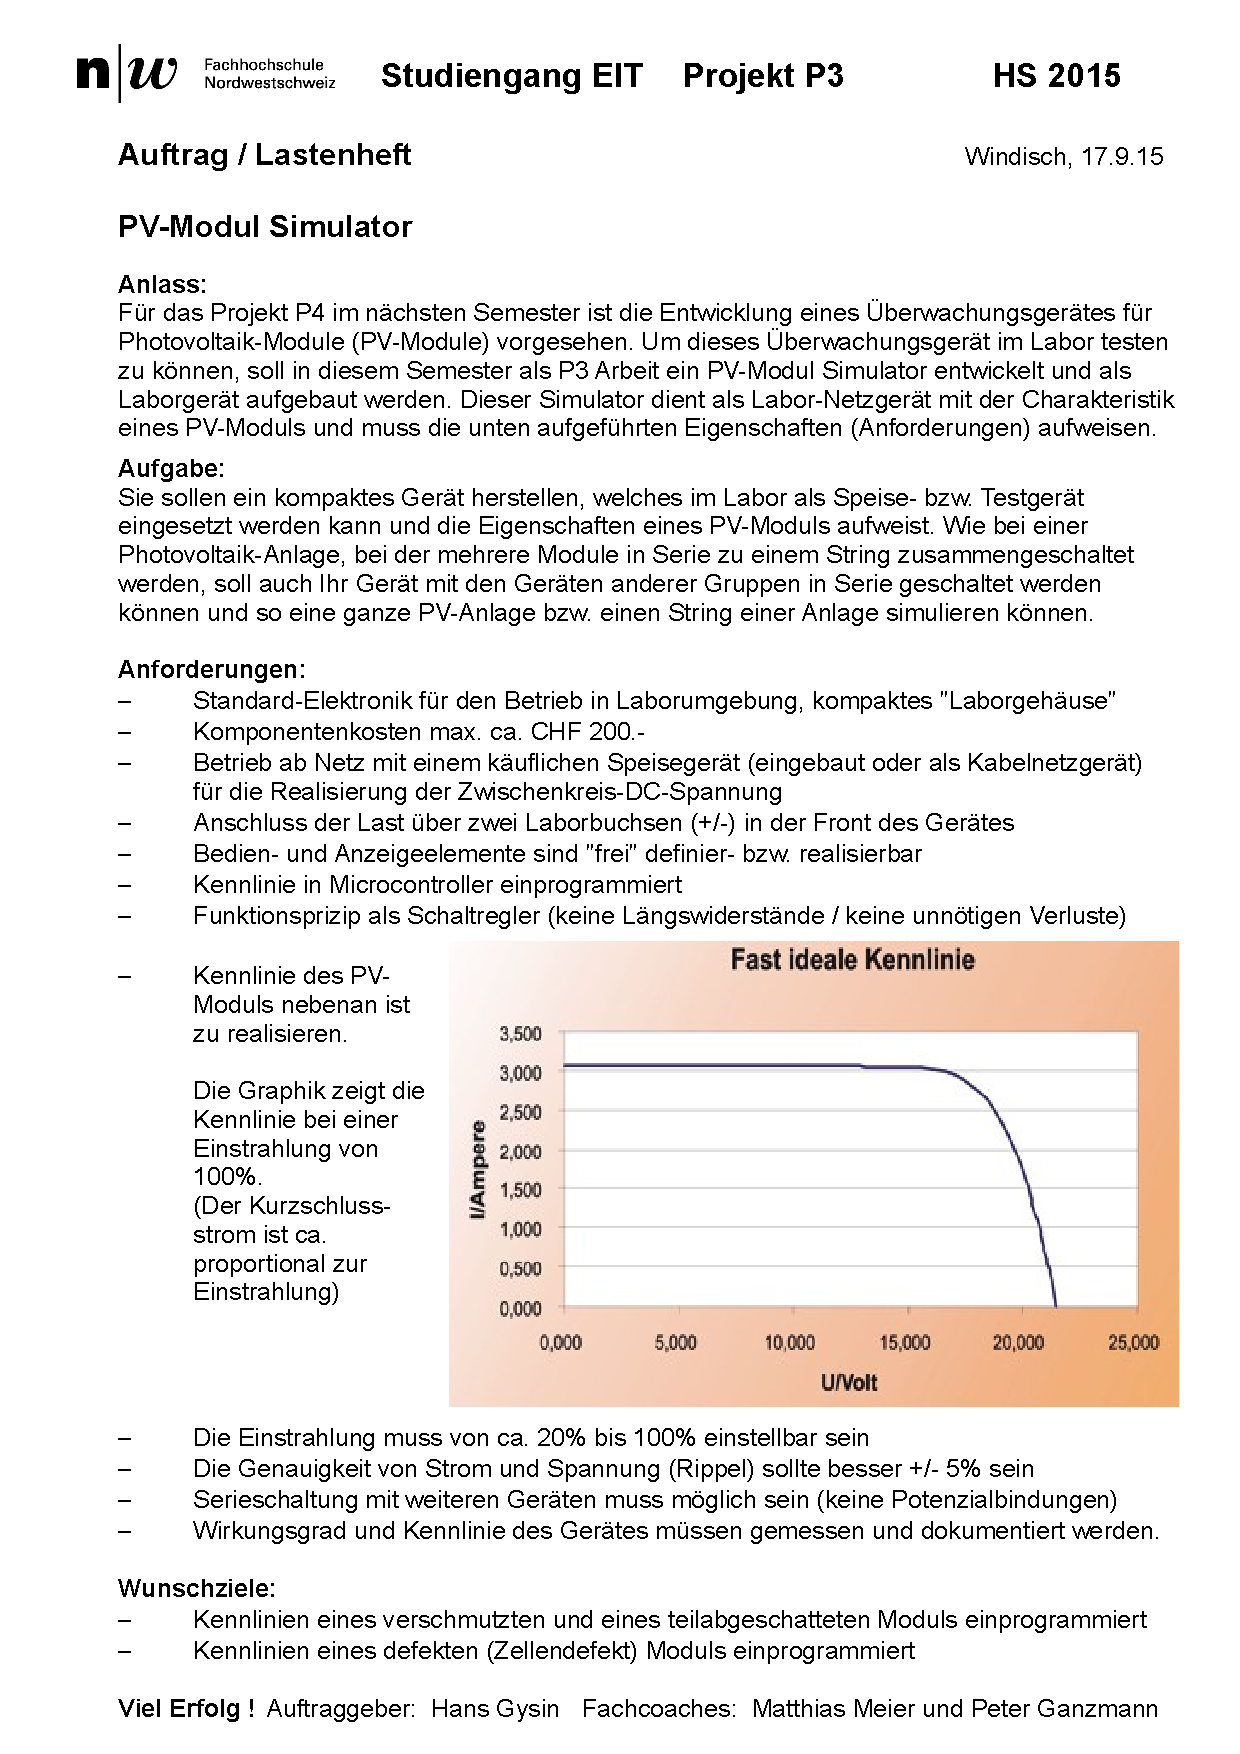
\includepdf[pages=-,scale=1]{images/specs.pdf}
%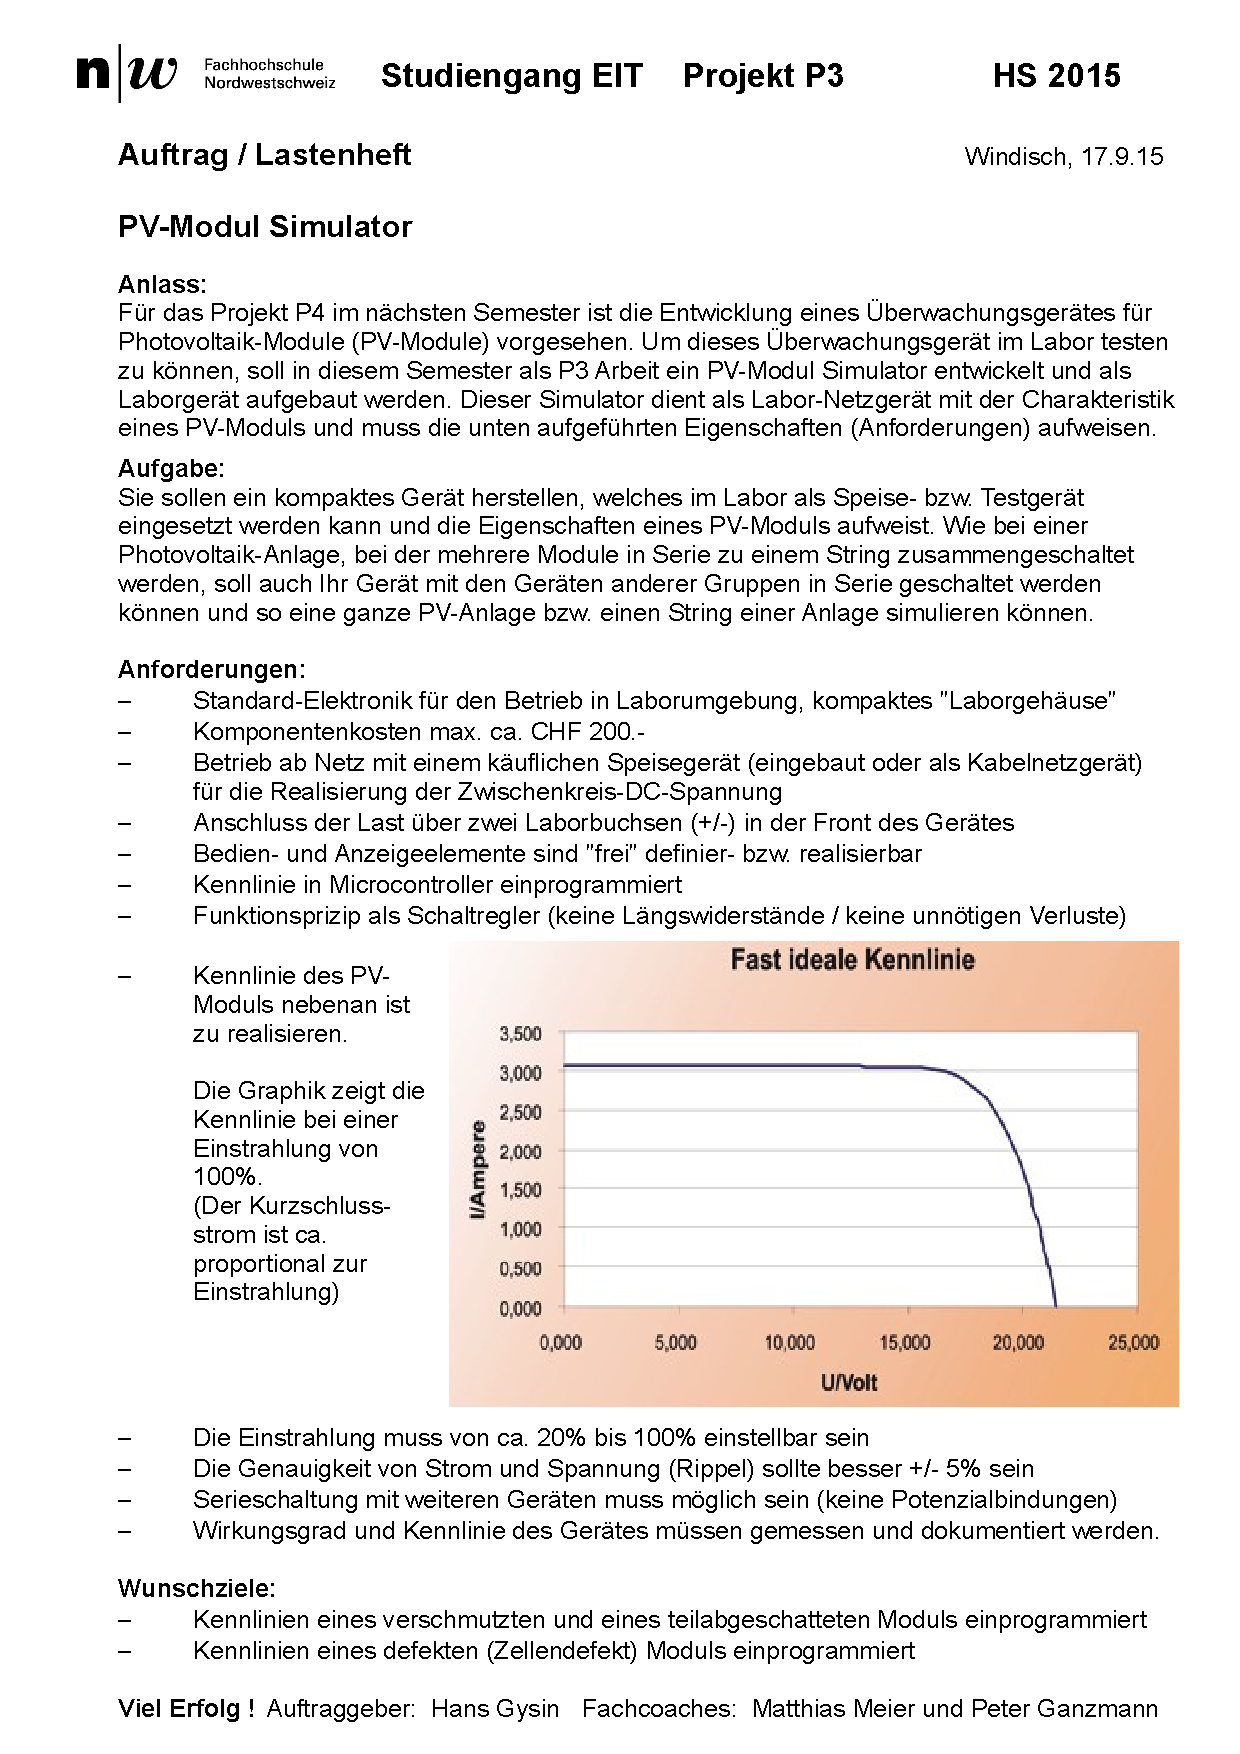
\includegraphics[width=\paperwidth]{images/specs.pdf}

{%START A3 PAGES
    \clearpage
    \pdfpagewidth=2\pdfpagewidth
    \textwidth=2\textwidth
    \addtolength{\textwidth}{50mm}

    % **************************************************************************** %
    \section{LT3471 Circuit}
    \label{appendix:lt3741:circuit}
    % **************************************************************************** %

    \begin{minipage}[b]{.45\textwidth}
        The   circuit    used   to    control   the   LT3471    is   described
        in   detail   in   section  \ref{subsec:lt3741}   starting   on   page
        \pageref{subsec:lt3741}. For the  reader's convenience,  the schematic
        in Figure \ref{fig:circuit:buck} is intended to be folded out and kept
        open as  a reference while  reading that section of  this report. This
        allows  for easy  cross-checking  between text  and schematic  without
        needing to constantly scroll through  the report's pages or needing to
        insert multiple copies of Figure \label{fig:circuit:buck}.
    \end{minipage}%
    \begin{minipage}[b]{.55\textwidth}
        \center
        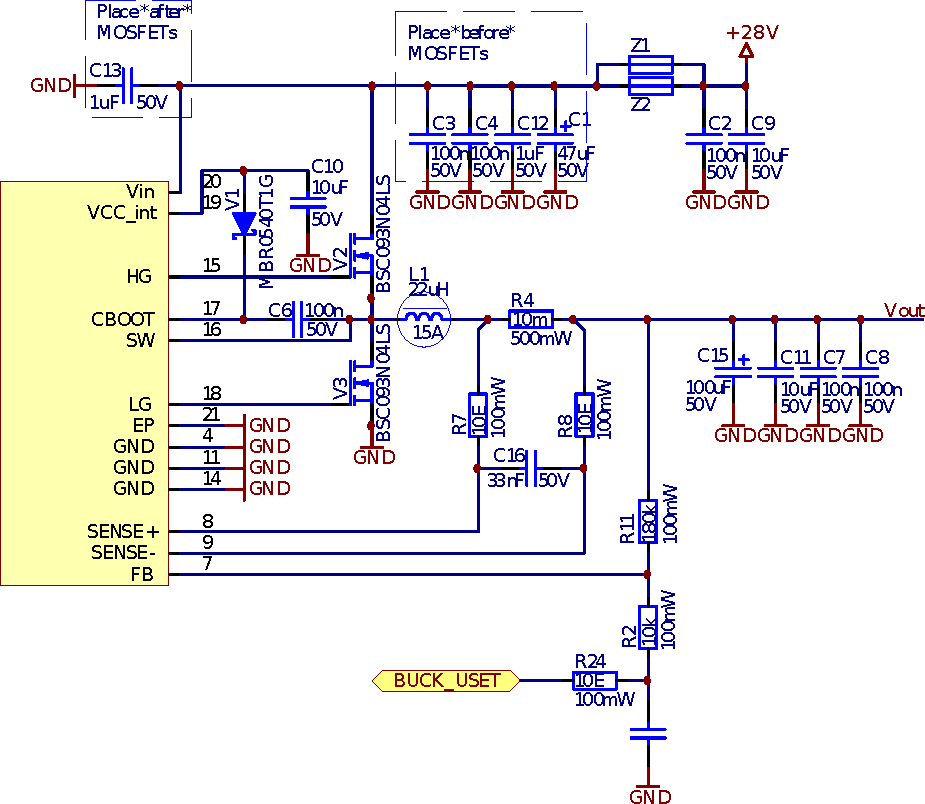
\includegraphics[width=.67\textwidth]{images/circuit/buck.pdf}
        %\caption{Herzst\"uck des Projektes: Aufbau des LT3741 CVCC Synchronwandler}
        \captionof{figure}{The device's heart: Overview of circuit for the LT3741 CCVC synchronous converter.}
        \label{fig:circuit:buck}
    \end{minipage}

\clearpage
}

\setlength\paperheight{297mm}
\setlength\paperwidth{420mm}
\setlength\pdfpageheight{\paperheight}
\setlength\pdfpagewidth{\paperwidth}

    % **************************************************************************** %
    \section{List of Components}
    \label{appendix:components}
    % **************************************************************************** %
    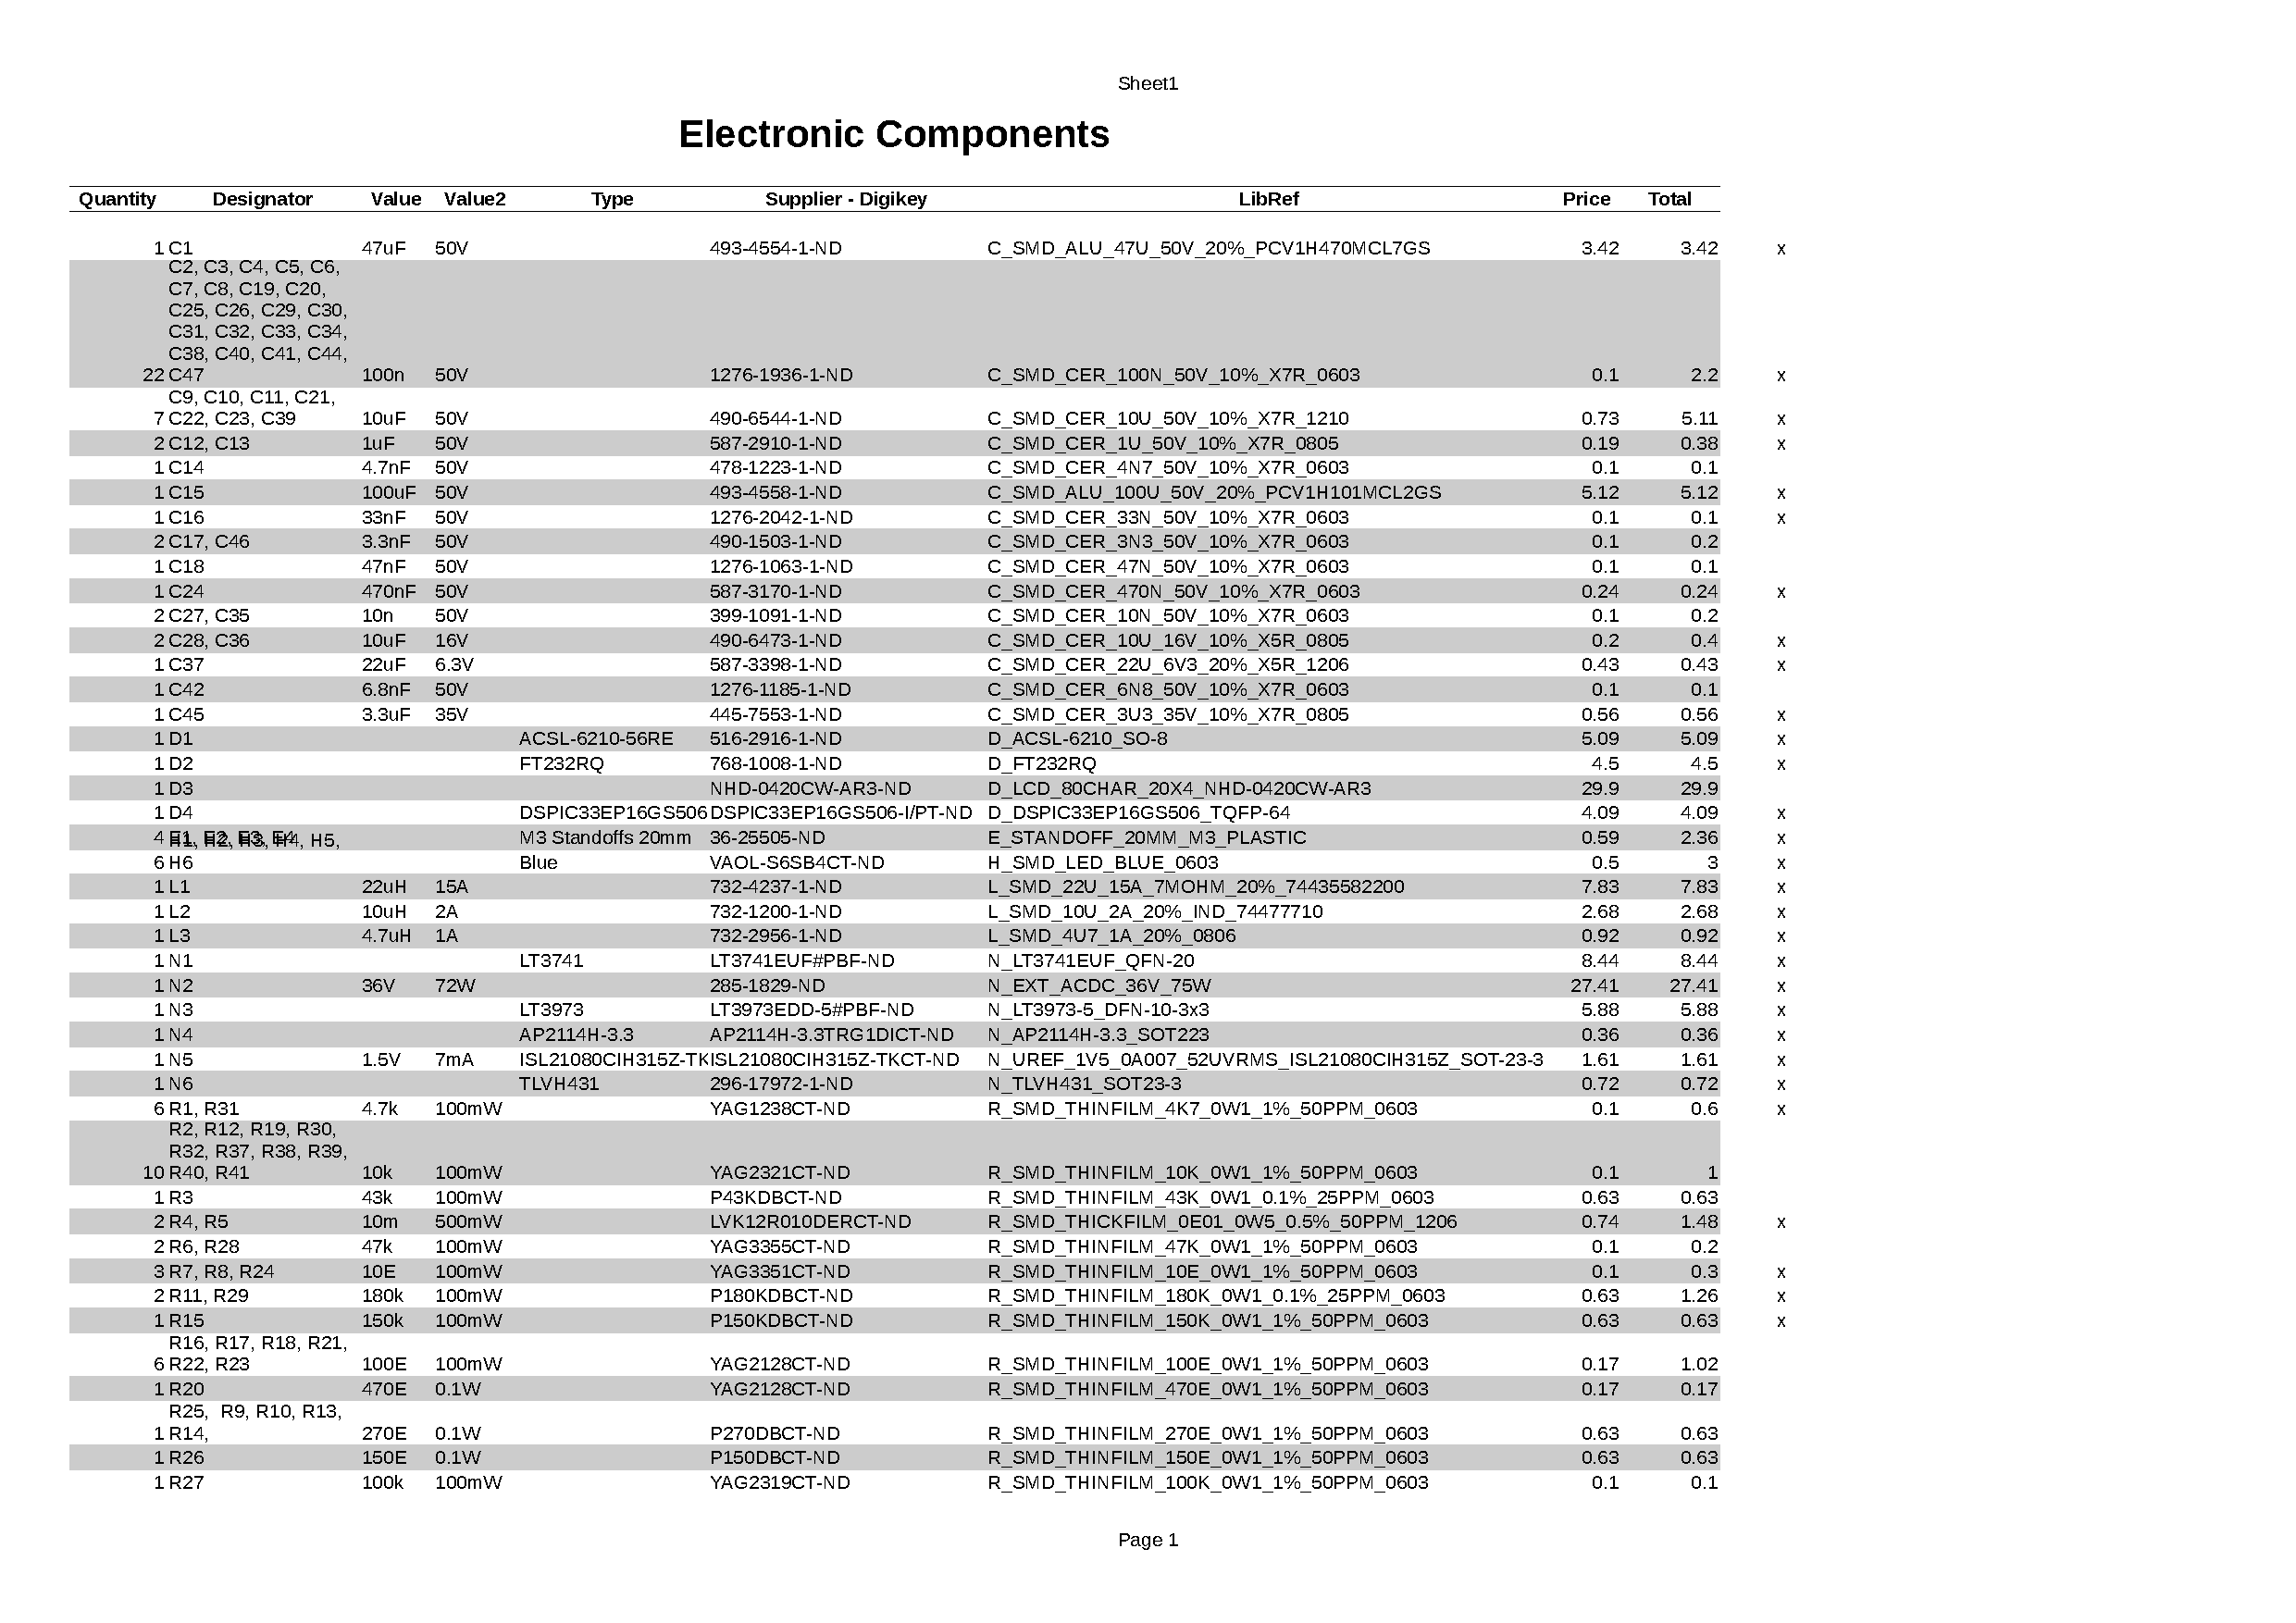
\includepdf[pages=-,scale=1]{images/bom.pdf}


    % **************************************************************************** %
    \section{Circuit Schematics}
    \label{appendix:schematics}
    % **************************************************************************** %
    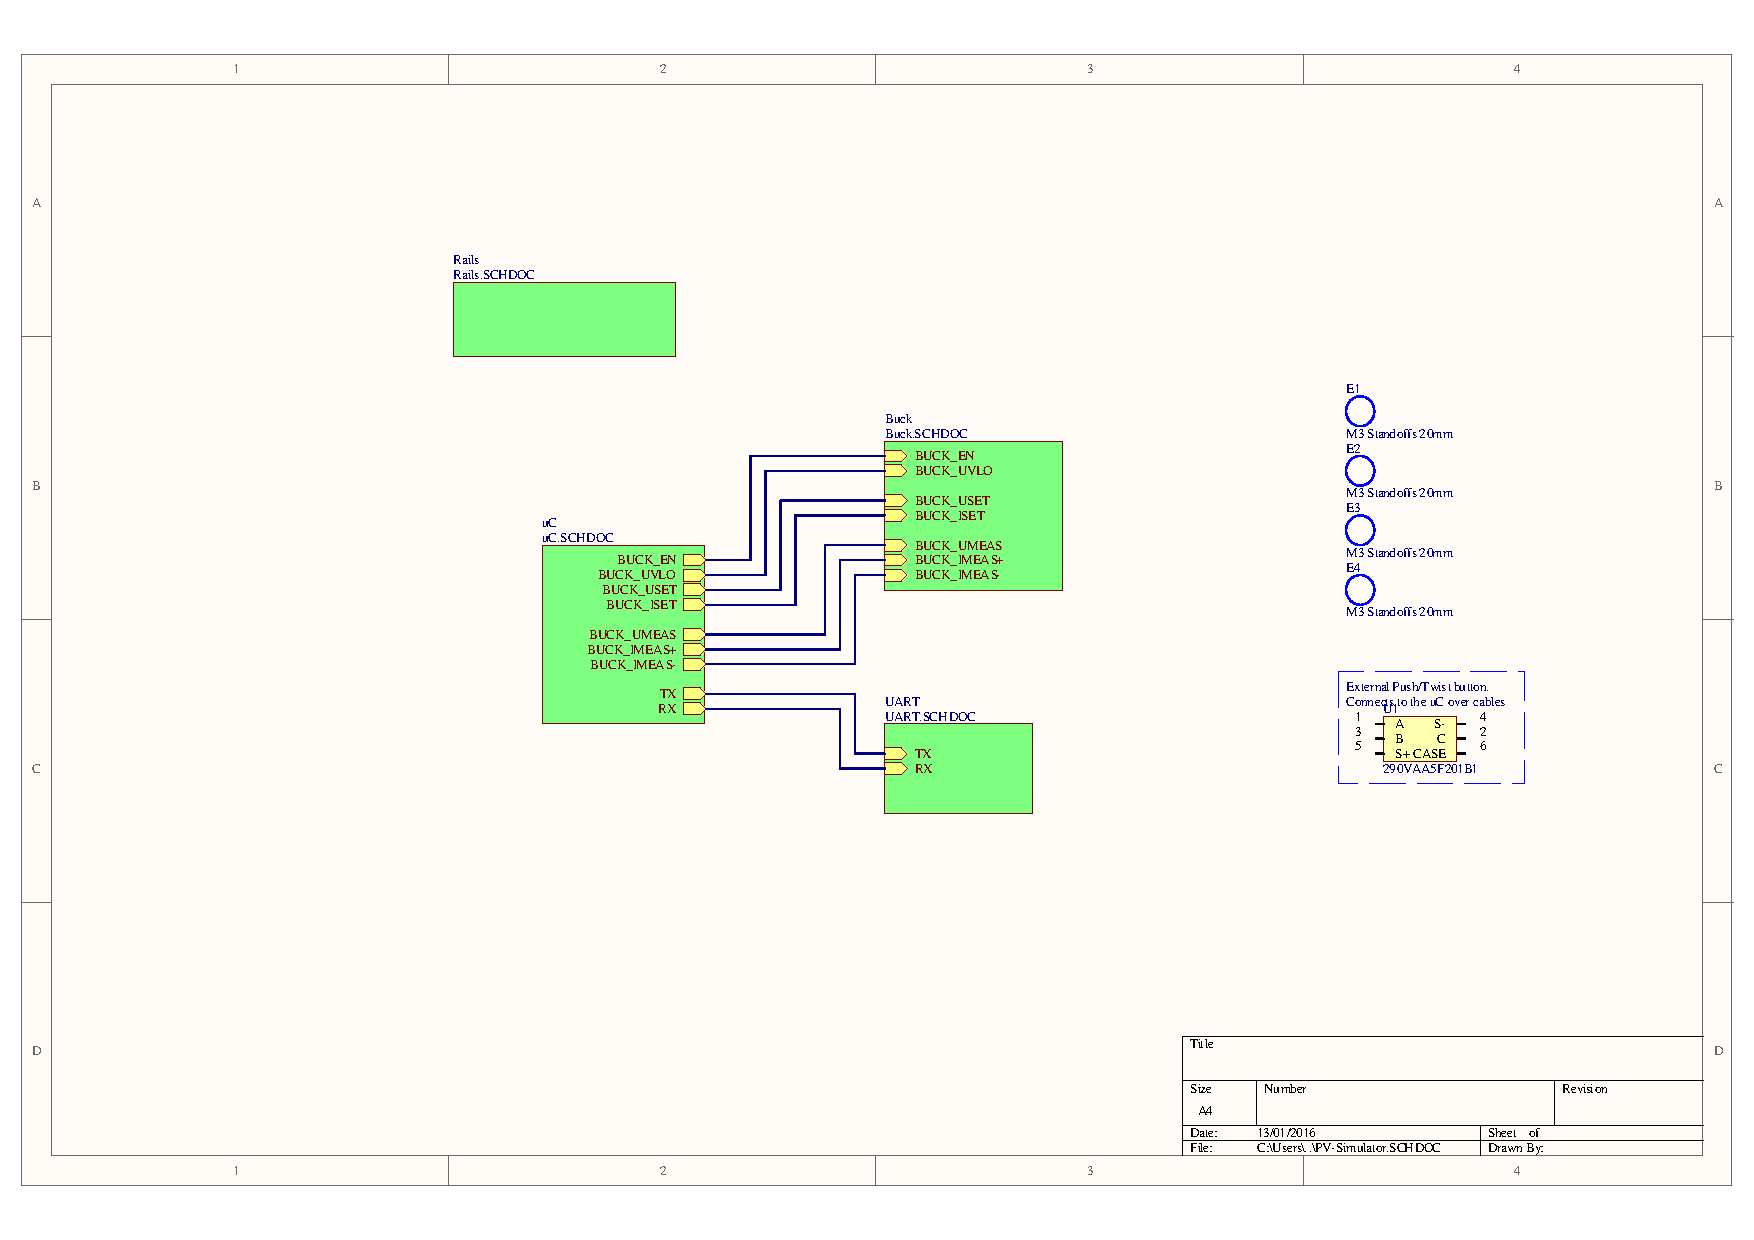
\includepdf[pages=-,scale=1]{images/schematic.pdf}

\setlength\paperheight{210mm}
\setlength\paperwidth{297mm}
\setlength\pdfpageheight{\paperheight}
\setlength\pdfpagewidth{\paperwidth}




% **************************************************************************** %
\clearpage
\section{Inductors}
\label{appendix:inductors}
% **************************************************************************** %

Filtering available  inductors according to  the criteria outlined  in section
\ref{subsubsec:lt3741:inductors} on  page \pageref{subsubsec:lt3741:inductors}
left us  with the models listed  in Table \ref{tab:circuit:buck:inductor}. The
model highlighted  in grey  was selected  due to it  having the  lowest direct
current resistance (DCR).

\begin{table}[th!]
    \begin{center}
        \caption{List of inductors matching our requirements}
        \label{tab:circuit:buck:inductor}
        \begin{tabular}{lcccc}
            \toprule
            Digikey         & Price (CHF) & Inductance (\SI{}{\micro\henry}) & DCR (\SI{}{\ohm}) & Ohmic Loss (\SI{}{\watt}) \\
            \midrule
            \rowcolor{lightgray}
            732-4237-1-ND   & 8.03        & 22                               & 0.007             & 0.175  \\
            732-2179-1-ND   & 6.4         & 47                               & 0.0335            & 0.8375 \\
            732-2177-1-ND   & 6.4         & 22                               & 0.0146            & 0.365  \\
            \bottomrule
        \end{tabular}
    \end{center}
\end{table}


% **************************************************************************** %
\section{MOSFETs}
\label{appendix:mosfets}
% **************************************************************************** %

Table     \ref{tab:circuit:buck:mosfet}     lists    MOSFETs     that     meet
the    constraints     outlined    in     \ref{subsubsec:lt3741:mosfets}    on
\pageref{subsubsec:lt3741:mosfets}.  For each one  the power losses $P_{LOSS}$
and $P_{LOSS\_LDO}$ were calculated.

\begin{table}[th!]
    \begin{center}
        \caption{Possible choices for MOSFETs}
        \label{tab:circuit:buck:mosfet}
        \begin{tabular}{cccccccccc}
            \toprule
            $R_{DS_{(on)}}$ & $Q_{GD}$ & $Q_{GS}$ & $R_G$ & $V_{GS_{THR}}$ & Ohmic Loss & Transision Loss & Total Loss & Drive Loss \\
            \midrule
            0.0032          & 4        & 2.5      & 0.4   & 2.5            & 0.104      & 1.0296          & 1.1336     & 0.806 \\
            0.0039          & 7        & 9        & 2.4   & 3.3            & 0.12675    & 4.8384          & 4.96515    & 1.984 \\
            0.0042          & 7        & 9        & 2.4   & 3.3            & 0.1365     & 4.8384          & 4.9749     & 1.984 \\
            0.008           & 2        & 4.5      & 3     & 2              & 0.26       & 2.2464          & 2.5064     & 0.558 \\
            0.0067          & 5.3      & 3.9      & 1.5   & 1              & 0.21775    & 2.18592         & 2.40367    & 0.7998 \\
            \rowcolor{lightgray}
            0.0093          & 2        & 4.9      & 1     & 2              & 0.30225    & 1.39104         & 1.69329    & 1.488 \\
            0.019           & 8        & 4        & 1.3   & 2              & 0.6175     & 2.6784          & 3.2959     & 1.798 \\
            0.0095          & 7.5      & 6        & 1     & 3              & 0.30875    & 2.7216          & 3.03035    & 1.736 \\
            \bottomrule
        \end{tabular}
    \end{center}
\end{table}


The MOSFET highlighted in grey was selected.  Though it is not the best model,
it is a lot  cheaper than the best fit and  has better documentation. The same
MOSFET is used for both the low-side and the high-side switch.


\end{appendices}

% **************************************************************************** %
\clearpage
\phantomsection
\addcontentsline{toc}{section}{\bibname}
\bibliography{bibliography/bibliography}{\bibliographystyle{bibliography/IEEEtrans.bst}}
% **************************************************************************** %
\end{document}
